\documentclass[11pt]{amsart}
%\usepackage[utf8]{inputenc}
\usepackage[UKenglish]{isodate}
\usepackage{amsmath}
\usepackage{amsthm}
\usepackage{amsbsy}
\usepackage{amssymb}
\usepackage{amsfonts}
\usepackage[dvips]{lscape}
\usepackage{xcolor}
\usepackage{amscd}
\usepackage[all,cmtip]{xy}
\usepackage{euscript}
\usepackage{parskip}
\usepackage{enumerate}
%\usepackage{fullpage}
\usepackage{yfonts}
\usepackage{xcolor}
\usepackage{graphicx}
\usepackage{fancyhdr}
\usepackage{tikz-cd}

\usepackage[margin=1in]{geometry}
\geometry{letterpaper}

\usepackage[expansion=false]{microtype}
\usepackage[pdfusetitle,unicode,hidelinks]{hyperref}

\theoremstyle{plain}


\setlength{\parskip}{0pt}
\setlength{\parsep}{0pt}
%\setlength{\headsep}{0pt}
%\setlength{\topskip}{0pt}
%\setlength{\topmargin}{0pt}
%\setlength{\topsep}{0pt}
%\setlength{\partopsep}{0pt}

\setcounter{tocdepth}{1}
\setlength{\parindent}{0in}

\theoremstyle{plain}
\newtheorem{theorem}{Theorem}[section]
\newtheorem{maintheorem}{Theorem}
\newtheorem{proposition}[theorem]{Proposition}
\newtheorem{lemma}[theorem]{Lemma}
\newtheorem{corollary}[theorem]{Corollary}
\newtheorem{notation}[theorem]{Notation}
\newtheorem{conjecture}[theorem]{Conjecture}

	\renewcommand{\vec}[1]{\mathbf{#1}}
\theoremstyle{remark}
\newtheorem{remark}[equation]{Remark}
\newtheorem{example}[theorem]{Example}
\newtheorem{question}[theorem]{Question}
\newtheorem{theoremA}{Theorem A}

\theoremstyle{definition}
\newtheorem{definition}[theorem]{Definition}

\newcommand{\Mod}{\mathcal{M}\textup{od}}
\newcommand{\Fun}{\textup{Fun}}
\newcommand{\Sp}{\mathcal{S}\textup{pt}}
\setcounter{tocdepth}{2}
\setlength{\parindent}{0in}
\newcommand{\Spec}{\textup{Spec}}
\newcommand{\Top}{\mathcal{T}\textup{opoi}}
\newcommand{\Sm}{\mathcal{S}\textup{m}}
\newcommand{\Shv}{\mathcal{S}\textup{hv}}
\newcommand{\PSh}{\mathcal{P}\textup{Sh}}
\newcommand{\Spc}{\mathcal{S}\textup{pc}}
\newcommand{\Spt}{\mathcal{S}\textup{pt}}
\newcommand{\Map}{\textup{Map}}
\newcommand{\et}{\textup{\'et}}
\newcommand{\Sym}{\textup{Sym}^{\infty}_{\bullet}}
\newcommand{\fSym}{\textup{Sym}_{\bullet}}
\newcommand{\Ext}{\textup{Ext}}
\newcommand{\Nis}{\textup{Nis}}
\newcommand{\Hom}{\textup{Hom}}
\newcommand{\Pro}{\textup{Pro}}
\newcommand{\gr}{\textup{gr}}
\newcommand{\D}{\textup{D}}
\newcommand{\DM}{\textup{DM}}
\newcommand{\Cat}{\mathcal{C}\textup{at}_{\infty}}
\newcommand{\id}{\textup{id}}
\newcommand{\Sch}{\mathcal{S}\textup{ch}}
\newcommand{\Ex}{\textup{Ex}}
\newcommand{\mathcalg}{\textup{CAlg}}
\newcommand{\Cato}{\Cat^{\otimes}}
\newcommand{\Var}{\textup{Var}}
\let\lim=\relax
\DeclareMathOperator*{\colim}{colim}
\DeclareMathOperator*{\lim}{lim}
\newcommand{\ord}{\textup{ord}}
\newcommand{\im}{\textup{im}}
\newcommand{\coker}{\textup{coker}}
\newcommand{\Perf}{\textup{Perf}}
\newcommand{\vdim}{\textup{vdim }}
\newcommand{\diag}{\textup{diag}}
\newcommand{\dcat}{D^b\textup{Coh}}
\newcommand{\Num}{\textup{Num}}
\newcommand{\Vect}{\textup{Vec}}
\newcommand{\Chow}{\textup{Chow}}
\newcommand{\SH}{\textup{SH}}
\newcommand{\SHeff}{\textup{SH}^{\textup{eff}}}
\newcommand{\SHconv}{\textup{SH}^{\textup{eff},\textup{conv}}}
\newcommand{\cdh}{\textup{cdh}}
\newcommand{\Zp}{\mathbb{Z}[1/p]}
\newcommand{\codim}{\textup{codim}}
\newcommand{\Fr}{\textup{Fr}}
\newcommand{\cl}{\textup{cl}}
\newcommand{\Lin}{\textup{Lin}}
\newcommand{\FT}{\textup{FT}}
\newcommand{\tr}{\textup{tr}}
\newcommand{\aff}{\textup{aff}}
\newcommand{\rad}{\textup{rad}'_3}


\renewcommand{\hat}{\widehat}
\newcommand{\Ki}{K_\infty}
\newcommand{\ki}{K_\infty}
\newcommand{\hQ}{\widehat{Q}}
\newcommand{\hP}{\widehat{P}}
\newcommand{\hR}{\widehat{R}}
\newcommand{\hY}{\widehat Y}
\newcommand{\hJ}{\widehat J}
\newcommand{\hJo}{\widehat{J_1}}
\newcommand{\het}{H_{\text{\'et}}}
\newcommand{\hYt}{\widehat{Y_2}}
\newcommand{\hl}{\widehat l}
\newcommand{\Kl}{\textup{Kl}}
\newcommand{\Sa}{\textup{Sa}}
\renewcommand{\div}{\textup{div}}



\newcommand{\PP}{\mathbb{P}}
\renewcommand{\AA}{\mathbb{A}}
\newcommand{\A}{\mathbf{A}}
\newcommand{\FF}{\mathbb{F}}
\newcommand{\ZZ}{\mathbb{Z}}
\newcommand{\ZZp}{\mathbb{Z}_{\mathrm{prim}}}
\newcommand{\NN}{\mathbb{Z}_{>0}}
\newcommand{\NNz}{\mathbb{N}_{\geq 0}}
\newcommand{\QQ}{\mathbb{Q}}
\newcommand{\RR}{\mathbb{R}}
\newcommand{\CC}{\mathbb{C}}
\newcommand{\EE}{\mathbb{E}}
\newcommand{\TT}{\mathbb{T}}
\newcommand{\PGL}{\textup{PGL}}
\newcommand{\PSL}{\textup{PSL}}
\newcommand{\Supp}{\textup{Supp}}

\newcommand{\sumstar}{\sideset{}{^*}\sum}

\newcommand{\cA}{\mathcal{A}}
\newcommand{\cS}{\mathcal{S}}
\newcommand{\cQ}{\mathcal{Q}}
\newcommand{\cD}{\mathcal{D}}
\newcommand{\cM}{\mathcal{M}}
\newcommand{\cW}{\mathcal{W}}
\newcommand{\cR}{\mathcal{R}}
\newcommand{\cP}{\mathcal{P}}
\newcommand{\cO}{\mathcal{O}}
\newcommand{\cF}{\mathcal{F}}
\newcommand{\cL}{\mathcal{L}}
\newcommand{\cG}{\mathcal{G}}
\newcommand{\vol}{\textup{vol}}
\newcommand{\exc}{\textup{exc}}



\newcommand{\Zell}{\mathbb{Z}_{(\ell)}}
\newcommand{\Four}{\textup{Four}}
\renewcommand{\contentsname}{}
\begin{document}
\title{Sections of quadrics over $\mathbb{A}^1_{\mathbb{F}_q}$}
\author{Naser T. Sardari and Masoud Zargar}

\address{Department of Mathematics, UW-Madison, Madison, WI 53706}
\email{ntalebiz@math.wisc.edu}

\address{Department of Mathematics, University of Regensburg, Regensburg, Germany}
\email{masoud.zargar@ur.de}


\renewcommand{\contentsname}{}

\begin{abstract}
Given finitely many closed points in distinct fibers of a non-degenerate quadric over $\mathbb{A}^1_{\mathbb{F}_q}$, we ask for conditions under which there is a section passing through the closed points, possibly with higher order (nilpotence) conditions. This is equivalent to proving strong approximation for non-degenerate quadrics over $\mathbb{F}_q[t]$.  We show that under mild conditions on the quadratic form $F$ over $\mathbb{F}_q[t]$ in $d$ variables, $f,g\in\mathbb{F}_q[t]$, $\boldsymbol{\lambda}\in\mathbb{F}_q[t]^d$, if $d\geq 5$ then for $\deg f\geq (4+\varepsilon)\deg g+O(1)$ we have a solution $\vec{x}\in\mathbb{F}_q[t]^d$ to $F(\vec{x})=f$ such that $\vec{x}\equiv\boldsymbol{\lambda}\bmod g$, where the the big-Oh notation does not depend on $f,g,\boldsymbol{\lambda}$. For $d=4$, we show the same is true for $\deg f\geq (6+\varepsilon)\deg g+O(1)$. In contrast to the $d=4$ case, our result is optimal for $d\geq 5$. This gives us a new proof (independent of the Ramanujan conjecture over function fields proved by Drinfeld) that the diameter of $k$-regular Morgenstern Ramanujan graphs $G$ is at most $2\log_{k-1}|G|+O(1)$ as $|G|\rightarrow\infty$. \footnotetext{\date\today}
\end{abstract}
\maketitle
\setcounter{tocdepth}{1}
\tableofcontents
\section{Introduction}\label{intro}
\subsection{Motivation}
We begin by considering a natural geometric problem regarding quadratic forms over $\mathbb{F}_q[t]$. Suppose $F$ is a quadratic form in $d$ variables over $\mathbb{F}_q[t]$. Suppose $f$ is a polynomial in $\mathbb{F}_q[t]$. We may then consider the affine variety $X_f$ given by setting $F(\vec{x})=f$, $\vec{x}\in\mathbb{A}^d_{\mathbb{F}_q[t]}$. We may view this as a family $\pi:X_f\rightarrow\mathbb{A}^1_{\mathbb{F}_q}$ over $\mathbb{A}^1_{\mathbb{F}_q}$. Suppose we have a collection of closed points $p_1,\hdots,p_m$ in $\mathbb{A}^1_{\mathbb{F}_q}$. Choose, for each $i$, a point $\boldsymbol{\lambda}_i:=(\lambda_1(p_i),\hdots,\lambda_d(p_i))$ in the fiber $X_{p_i}:=X_f\times_{\mathbb{F}_q[t]}\kappa(p_i)$ over $p_i$.  Can we find a section $s:\mathbb{A}^1_{\mathbb{F}_q}\rightarrow X_f$ of the structure morphism $\pi:X_f\rightarrow\mathbb{A}^1_{\mathbb{F}_q}$ that maps each $p_i$ to $\boldsymbol{\lambda}_i$ with some prescribed higher order (nilpotence) conditions of order $m_i$? We show that if $F$ is non-degenerate in $d\geq 5$ variables, then there is such a section provided that $\deg f \geq (4+\varepsilon)\sum_{i}m_i\deg p_i +O_{\varepsilon,F}(1)$, where the implied constant depends only on $\varepsilon$ and the quadratic form $F$ (in fact, we show a stronger result depending on anisotropic cones defined in definition~\ref{def:aniso}). We also show that this condition is optimal. On the other hand, if $d=4$, we show that this is true at least if $\deg f\geq (6+\varepsilon)\sum_{i}m_i\deg p_i+O_{\varepsilon,F}(1)$. That being said, we conjecture that  $4+\varepsilon$ still suffices in the $d=4$ case. In fact, as will appear in a future paper, we will show that the optimality of $4+\varepsilon$ when working with the class of quadratic forms in the construction of Morgenstern Ramanujan graphs follows from a twisted Linnik-Selberg conjecture over function fields. The setup of the problem is pictorially represented by the following figure.
\[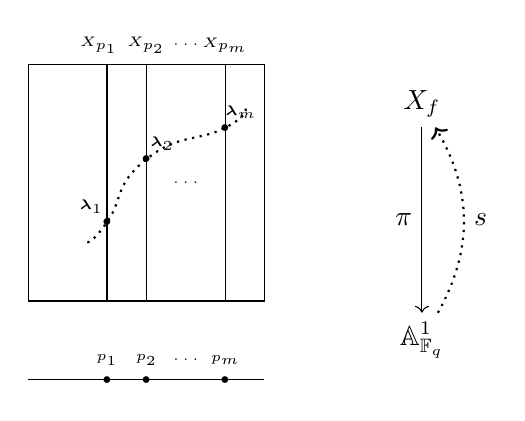
\begin{tikzpicture}

\draw (0,0) rectangle (3,3);
\node (A) at (5,2.5) {$X_f$};
\draw (0,-1)--(3,-1);
\node (B) at (5,-0.5) {$\mathbb{A}^1_{\mathbb{F}_q}$};
\draw [->] (A) to node[left]{$\pi$} (B);
\draw [bend right, ->, dotted, thick] (B) to node[right]{$s$}(A);
\draw (1,-0.75) node{\tiny $p_1$};
\draw (1.5,-0.75) node{\tiny $p_2$};
\draw (2,-0.75) node{\tiny $\hdots$};
\draw (2.5,-0.75) node{\tiny $p_m$};
\draw (1,-1) node{\tiny $\bullet$};
\draw (1.5,-1) node{\tiny $\bullet$};
\draw (2.5,-1) node{\tiny $\bullet$};
\draw (1,0)--(1,3);
\draw (1.5,0)--(1.5,3);
\draw (2.5,0)--(2.5,3);
\draw (2,1.5) node{\tiny $\hdots$};
\draw (0.8,1.2) node{\tiny $\boldsymbol{\lambda}_1$};
\draw (1.7,2) node{\tiny $\boldsymbol{\lambda}_2$};
\draw (2.7,2.4) node{\tiny $\boldsymbol{\lambda}_m$};
\draw (1,1) node{\tiny $\bullet$};
\draw (1.5,1.8) node{\tiny $\bullet$};
\draw (2.5,2.2) node{\tiny $\bullet$};

\draw [thick, dotted] plot [smooth, tension=1] coordinates { (0.75,0.75) (1,1) (1.5,1.8) (2.5,2.2) (2.75,2.45)};

\draw (0.9,3.25) node{\tiny $X_{p_1}$};
\draw (1.5,3.25) node{\tiny $X_{p_2}$};
\draw (2,3.25) node{\tiny $\hdots$};
\draw (2.5,3.25) node{\tiny $X_{p_m}$};
\end{tikzpicture}\]
There is another more algebraic way of formulating the problem; in fact, this other formulation is more common. By packaging all the closed points $p_i$ and all their multiplicities $m_i>0$ (which can be viewed as irreducible polynomials $p_i(t)$ in $\mathbb{F}_q[t]$ raised to the power of $m_i$) into one polynomial $g(t):=\prod_ip_i(t)^{m_i}$, we can use the Chinese remainder theorem to reformulate the problem as an optimal strong approximation problem for quadratic forms over function fields. More precisely, we ask for the following. Suppose we have a quadratic form $F$ in $d$ variable over $\mathbb{F}_q[t]$, and polynomials $g,f\in\mathbb{F}_q[t]$. Additionally, we are given polynomials $\lambda_1,\hdots,\lambda_d\in\mathbb{F}_q[t]$. We want to know when we have an integral solution $\vec{x}:=(x_1,\dots,x_d)\in \mathbb{F}_q[t]^d $ to the system
\begin{equation}\label{maineq}\begin{cases}F(\vec{x})=f,\\ \vec{x}\equiv\boldsymbol{\lambda}\bmod g,\end{cases}\end{equation}
where $\boldsymbol{\lambda}=(\lambda_1,\dots,\lambda_d)$ and $\vec{x}\equiv\boldsymbol{\lambda}\bmod g$ means $x_i\equiv \lambda_i\bmod g$ for every $1\leq i\leq d$. For a prime ideal $\varpi$  of  ${\mathbb{F}_q[t]},$ we write ${\mathbb{F}_q[t]}_{\varpi}$ for the completion of $\mathbb{F}_q[t]$ at $\varpi$. We say all local conditions for the system~\eqref{maineq} are satisfied, if $F(x) = f$ has a
local solution $\vec{x}_{\varpi} \in  {\mathbb{F}_q[t]}_{\varpi}^d$ for all prime ideals  $\varpi$ of  $\mathbb{F}_q[t]$ (Here, $\mathbb{F}_q[t]_{\varpi}$ is the completion of $\mathbb{F}_q[t]$ at the prime $\varpi$) such that $\vec{x}_{\varpi}\equiv\boldsymbol{\lambda}\bmod \varpi^{\ord_{\varpi}(g)}.$ In the following $K_{\infty}:=\mathbb{F}_q(\!(1/t)\!)$, $\widehat{(-)}:=q^{(-)}$. $K_{\infty}^d$ is equipped with the norm $|\vec{x}|:=\max_i|x_i|$ for any $\vec{x}=(x_1,\hdots,x_d)\in K_{\infty}^d$. Consider the following definition.
\begin{definition}[Anisotropic cone]\label{def:aniso}We say $\Omega\subset K_{\infty}^d$ is an anisotropic cone with respect to quadratic form $F(\vec{x})$ if there exists fixed positive integers $\omega$  and  $\omega^{\prime}$ such that: 

\begin{enumerate}
\item If $\vec{x}\in \Omega$ then $f\vec{x}\in \Omega$ for every $f\in K_\infty.$
\item \label{prop2} If $\vec{x}\in\Omega$ and $\vec{y} \in  K_\infty^d $ with $|\vec{y}|\leq |\vec{x}|/ \hat{\omega},$ then $\vec{x}+\vec{y} \in \Omega.$ 
\item \label{prop3}  $ \hat{\omega^{\prime}} |F(\vec{x})| \geq |\vec{x}|^2.$
\end{enumerate}
\end{definition}
The main result of this paper is the following theorem.
\begin{theorem}
\label{mainthm}Suppose $q$ is a power of a fixed odd prime number, and let $F$ be a non-degenerate quadratic form over $\mathbb{F}_q[t]$ in $d\geq 4$ variables and of discriminant $\Delta$. Let $f, g\in\mathbb{F}_q[t]$ be nonzero polynomials such that $(f\Delta,g)=1$, and let $\boldsymbol{\lambda}\in\mathbb{F}_q[t]^d$ be a $d$-tuple of polynomials at least one of whose coordinates is relatively prime to $g$. Finally, suppose that 
all local conditions for the system~\eqref{maineq}
are satisfied.  If $d\geq 5$, then for any anisotropic cone $\Omega$ and for $\deg f \geq (4+\varepsilon)\deg g +O_{\varepsilon,F,\Omega}(1)$,  there is a solution $\vec{x} \in \Omega\cap\mathbb{F}_q[t]^d $ to \eqref{maineq}. If $d=4$, this holds at least for $\deg f \geq (6+\varepsilon)\deg g +O_{\varepsilon,F,\Omega}(1).$
 \end{theorem}
\begin{remark}\label{optimality}For $F(\vec{x})=x_1^2+\hdots+x_d^2$, we can take $\Omega=\{\vec{x}\in K_{\infty}^d:\forall i,\ \deg x_1>\deg x_i\}$. Note that when $\deg f\leq 4\deg g-3$, then the system need not have a solution in $\mathbb{F}_q[t]^d\cap\Omega$. For instance, when $\boldsymbol{\lambda}=(1,0,\hdots,0)$ and $f\equiv 1+2t^{\deg g -1}g\bmod g^2$, then a solution implies the existence of $(t_1,\hdots,t_d)\in\mathbb{F}_q[t]^d$ such that
\[(1+t_1g)^2+(t_2g)^2+\hdots+(t_dg)^2\equiv 1+2t^{\deg g-1}g\bmod g^2, \]
that is, $t_1\equiv t^{\deg g-1}\bmod g$. Since the solution is in $\Omega$, the degree of $f$ is equal to the degree of $(1+t_1g)^2$, and so $\deg f\geq 2(2\deg g-1)=4\deg g-2$. This shows that the factor $4+\varepsilon$ is optimal.
\end{remark}
Another motivation for the consideration of this problem is the construction of Ramanujan graphs with optimal diameters. We begin by defining Ramanujan graphs. Fix an integer $k\geq 3$, and let $G$ be a $k$-regular connected graph with the adjacency matrix  $A_G.$ It follows that $k$ is an eigenvalue of $A_G$. Let $\lambda_G$ be the maximum of the absolute value of all the other eigenvalues of $A_G$. By the Alon-Boppana Theorem~\cite{Lubotzky1988}, $\lambda_G\geq 2\sqrt{k-1}+o(1)$, where $o(1)$ goes to zero as $|G|\to \infty$.  We say that $G$ is a Ramanujan graph if  $\lambda_G \leq 2\sqrt{k-1}.$\\
\\
The first explicit construction of Ramanujan graphs is due to Lubotzky-Phillips-Sarnak~\cite{Lubotzky1988}, and independently by Margulis \cite{Margulis}. It is a Cayley graph of $\PGL_2(\mathbb{Z}/q\mathbb{Z})$ or $\PSL_2(\mathbb{Z}/q\mathbb{Z})$ with $p+1$ explicit generators for every prime $p$ and integer $q$.   The optimal spectral gap on the LPS construction is a consequence of the Ramanujan bound on the Fourier coefficients of the weight 2 holomorphic modular forms, which justifies their naming. 
  We refer the reader to \cite[Chapter 3]{Peter}, where a complete history of the construction of Ramanujan graphs and other extremal properties of them are recorded. In particular, Lubotzky-Phillips-Sarnak proved that the diameter of every $k$-regular Ramanujan graph $G$ is bounded by $2\log_{k-1}|G|+O(1).$ This is still the best known upper bound on the diameter of a Ramanujan graph. It was conjectured that the diameter is bounded by $(1+\varepsilon)\log_{k-1}|G|$ as $|G|\to \infty;$ see \cite[Chapter 3]{Peter}. However, the first author proved that for some infinite families of LPS Ramanujan graphs the diameter is bigger than $4/3 \log_{k-1}|G|+O(1);$ see \cite{Sardari2018}. The first author has conjectured that the diameter of the LPS Ramanujan graphs is asymptotically $4/3 \log_{k-1}|G|+O(1)$, which would follow from an optimal strong approximation conjecture for integral quadratic forms in 4 variables; see \cite[Conjecture 1.3]{Naser2}. The following theorem of Lubotzky-Phillips-Sarnak  links the diameter of the LPS Ramanujan graphs to the strong approximation on the sphere.   
\begin{theorem}[Due to Lubotzky-Phillips-Sarnak \cite{Lubotzky1988}]\label{reductionthm} 
Let $v:=\begin{bmatrix} a_1 &a_2 \\ a_3 &a_4   \end{bmatrix} \in G$, where $G$ is the LPS Ramanujan graph associated to $p$ and $q$. There is a bijection between  non-backtracking  paths $(v_0,\dots,v_h)$  of length $h$ from $v_0=id$ to $v_h=v$  in $G$, and the set of integral solutions to the following diophantine equation 
\begin{equation}\label{redd}
\begin{split}
&x_1^2+x_2^2+x_3^2+x_4^2=N,
\\
&\begin{bmatrix}x_1+ix_2 & x_3+ix_4 \\ -x_3-ix_4 &x_1-ix_2 \end{bmatrix}  \equiv  \lambda \begin{bmatrix} a_1 &a_2 \\ a_3 &a_4   \end{bmatrix}  \text{ mod } 2q \text{ for some }\lambda \in \mathbb{Z}/2q,
\end{split}
\end{equation} 
   where $N=p^h$.
In particular, the distance between $id$ and $v$ in $G$ is the smallest exponent $h$ such that~\eqref{redd} has an integral solution. 
\end{theorem}
We state a version of the optimal strong approximation conjecture for the sphere, which when combined with this theorem implies that the diameter of LPS Ramanujan graphs is asymptotically $4/3 \log_{k-1}|G|+O(1);$ see \cite{Cayley, Complexity} for further numerical evidence on this conjecture.
\begin{conjecture}\label{mainconjecture}
Suppose that $N$, $m$ and $\lambda_1, \dots, \lambda_4$ are given integers such that 
$$
N\equiv \sum_{i=1}^4 \lambda_i^2 \mod m.
$$ 
Assuming that $N\gg m^{4+\varepsilon}$, there exists an integral solution $(x_1,\dots,x_4)$ to the system
\begin{equation*}\label{redd}
\begin{split}
&x_1^2+x_2^2+x_3^2+x_4^2=N,
\\
&x_l\equiv \lambda_l \text{ mod } m \text{ for  $1\leq l \leq 4$. }
\end{split}
\end{equation*} 
\end{conjecture}
 This conjecture is inspired by the conjecture of Sarnak on the distribution of integral points on the sphere $S^3$. Indeed, given $R>0$ such that $R^2\in \mathbb{Z}$, we let $C(R)$ denote the maximum volume  of any cap on  the $(d-1)$-dimensional sphere $S^{d-1}(R)$ of radius $R$ which contains no integral points. Sarnak defined  \cite{Sarnak2}
 the covering exponent of integral points on the sphere by:
 \begin{equation*}
 \begin{split}
 K_d&:=\limsup_{R \to \infty}\frac{\log \left(\# S^{d-1}(R)\cap \mathbb{Z}^d \right) }{\log\left( \text{vol } S^{d-1}(R)/C(R)\right)}.
 \end{split}
 \end{equation*}
 
In his letter \cite{Sarnak2} to  Aaronson and  Pollington, Sarnak showed that $4/3\leq K_4 \leq 2$. To show that $K_4\leq 2$, he appealed to the Ramanujan bound on the Fourier coefficients of weight $k$ modular forms, while the lower bound $4/3\leq K_4$ is a consequence of an elementary number theory argument. Furthermore, Sarnak states some open problems \cite[Page $24$]{Sarnak2}.  The first one is to show that  $K_4<2$ or  even that $K_4=4/3$.\\
\\
It follows from Theorem 1.8 and Corollary 1.9 of \cite{Naser2} that $K_d=2-\frac{2}{d-1}$ for $d\geq 5$ and $4/3\leq K_4 \leq 2$; see also \cite{Siegel} for bounds on the average covering expoent.  Browning-Kumaraswamy-Steiner~\cite{BKS} showed that $K_4 = 4/3$, subject to the validity of a twisted version of a conjecture of Linnik about cancellation in sums of Kloosterman sums; see also Remark 6.8 of \cite{Naser2}. We have shown, as will appear in a forthcoming paper, that a twisted version of the Linnik-Selberg conjecture proves the optimal bound for the diameter of Morgenstern Ramanujan graphs. Since the untwisted version of the Linnik-Selberg conjecture over function fields has already been proved using the Ramanujan conjecture over function fields (proved by Drinfeld), we are hopeful that we would be able to prove the desired twisted version of the conjecture. We will discuss this connection in a future paper.


\section{The delta method for small target}\label{deltamethod}
In this section, we define a weighted sum $N(w, \boldsymbol{\lambda})$ counting the number of integral solutions our problem. We then use the delta method to give an expression for it in terms of exponential sums and oscillatory integrals. This is done by giving an expansion of the delta function using the decomposition of $\TT$ (that we shall define below) found in the paper \cite{Browning} of Browning and Vishe. In this section, we also set up the basic notation that we shall use in this paper.

\subsection{Notation}
Let $K=\mathbb{F}_q(t)$ and let $\mathcal{O}=\mathbb{F}_q[t]$ be its ring of integers. Let $\Omega$ be its set of places of $K$. These correspond to either monic irreducible primes $\varpi$ in $\mathcal{O}$, called finite primes, or the prime at infinity $t^{-1}$ which we designate by $\infty$. The norms are given by
\[|a/b|_{\varpi}:=(q^{-\deg\varpi})^{\ord_{\varpi}(a/b)}\]
and
\[|a/b|_{\infty}:=q^{\deg a-\deg b}.\]
For every $d$ and place $v$, we define the natural norm on $K_v^d$ by $|\mathbf{a}|_v:=\max_i|a_i|_v$. Given $\mathbf{a}\in K_v^d$ and $r>0$, we define the closed ball $B_v(\mathbf{a},r):=\{\mathbf{x}\in K_v^d:|\mathbf{x}-\mathbf{a}|_v\leq r\}$. These furnish $K_v^d$ and $\mathcal{O}_v^d$ with topologies.\\
\\
We define the integral ring of adeles for $K^d$ as $\mathbf{A}^d_{\mathcal{O}}:=K_{\infty}^d\times\prod_{\varpi\neq\infty}\mathcal{O}_{\varpi}^d$. A \textit{global} ball in $\mathbf{A}^d_{\mathcal{O}}$ is defined to be the product of local balls subject to the condition that the radii of the local balls are $1$ for all but finitely many of them. If we have a global ball
\[B_{\mathbf{a},\mathbf{r}}:=B_{\infty}(\mathbf{a}_{\infty},r)\times\prod_{\varpi\neq\infty}B_{\varpi}(\mathbf{a}_{\varpi},(q^{-\deg\varpi})^{\nu_{\varpi}}),\]
$\nu_{\varpi}\geq 0$, the condition on the radii ensures that $m:=\prod_{\varpi}\varpi^{\nu_{\varpi}}$ is well-defined. We define the norm $|B_{\mathbf{a},\mathbf{r}}|$ to be $rm^{-1}\in K$.\\
We may identify $K_\infty$ with the field
$$
\FF_q(\!(1/t)\!)=\left\{\sum_{i\leq N}a_it^i: \mbox{for $a_i\in \FF_q$ and some $N\in\ZZ$} \right\}
$$
and put 
$$
\TT=\{\alpha\in K_\infty: |\alpha|<1\}=\left\{\sum_{i\leq -1}a_it^i: \mbox{for $a_i\in \FF_q$}
\right\}.
$$
Let  $\delta\in \TT$. Then $\TT/\delta\TT$ is the set of cosets $\alpha+\delta \TT$, of which there are  
$|\delta|.$\\
\\
In the function field setting, smooth functions $f:F\rightarrow\mathbb{C}$ from a non-archimedian local field $F$ are precisely the locally constant functions. The analogue here of Schwarz functions in real analysis is the notion of Schwarz-Bruhat functions which are the smooth (locally constant) functions $f:F\rightarrow\mathbb{C}$ with compact support. We denote the set of Schwarz-Bruhat functions on $F$ by $S(F)$. We can then extend this notion to Schwarz-Bruhat functions on $F^n$ by defining such a function to be one that is a Schwarz-Bruhat function in each coordinate. We could similarly define the space of Schwarz-Bruhat functions $S(\mathbf{A}^n_F)$ on the adeles $\mathbf{A}^n_F$.

\subsection{Characters}\label{s:add-characters}
There is a non-trivial additive character $e_q:\FF_q\rightarrow \CC^*$ defined
for each $a\in \FF_q$ by taking 
$e_q(a)=\exp(2\pi i \tr(a)/p)$, where $\tr: \FF_q\rightarrow \FF_p$ denotes the
trace map.
This character induces a non-trivial (unitary) additive character $\psi:
K_\infty\rightarrow \CC^*$ by defining $\psi(\alpha)=e_q(a_{-1})$ for any 
$\alpha=\sum_{i\leq N}a_i t^i$ in $\Ki$. In particular it is clear that
$\psi|_\cO$ is trivial. 
More generally, given any $\gamma \in \Ki$, the map $\alpha\mapsto \psi(\alpha\gamma)$ is an additive
character on $\Ki$. We then have the following orthogonality property.
\begin{lemma}[Kubota, Lemma 7 of
\cite{kubota}]\label{lem:orthogsum}
$$
\sum_{\substack{b\in \cO\\ |b|<\hat N}}\psi(\gamma b)=\begin{cases}
\hat N, & \mbox{if $|(\!(\gamma)\!)|<\hat N^{-1}$,}\\
0, & \mbox{otherwise},
\end{cases}
$$
for any $\gamma \in \ki$ and any integer $N\geq 0$, where $(\!(\gamma)\!)$ is the part of $\gamma$ with all degrees negative.
\end{lemma}
We also have the following
\begin{lemma}[Kubota, Lemma 1(f) of \cite{kubota}]\label{lem:orthog}
Let $Y\in \ZZ$ and $\gamma\in  \ki$. Then 
$$
\int_{|\alpha|<\hat{Y}} \psi(\alpha \gamma) d \alpha=\begin{cases}
\hat Y, &\mbox{if $|\gamma|<\hat Y^{-1}$},\\
0, &\mbox{otherwise.}
\end{cases}
$$
\end{lemma}
In particular, if we set $Y=0$, then we obtain the following expression for the delta function on $\mathcal{O}$:
\[\delta(x)=\int_{\TT}\psi(\alpha x)d\alpha,\]
where 
\[
\delta(x)=\begin{cases} 1 &\text{ if } x=0,\\ 0 &\text{ otherwise.}  \end{cases}
\]
\subsection{The delta function}The idea now is to decompose $\TT$ into a disjoint union of balls (with no minor arcs) which is the analogue of Kloosterman's version of the circle method in this function field setting. This is done via the following lemma of Browning and Vishe \cite[Lemma~4.2]{Browning}.
\begin{lemma}\label{lem:dissection}
For any $Q>1$ we have a disjoint union 
\[
\TT=\bigsqcup_{\substack{r\in \cO\\ |r|\leq \hat Q\\
\text{$r$ monic}}}
\bigsqcup_{\substack{a\in \cO\\ |a|<|r|\\ (a,r)=1} }
\left\{\alpha\in \TT: |r\alpha-a|<\hat Q^{-1}\right\}.\]
\end{lemma}
The following follows from Lemma \ref{lem:dissection}.
\begin{lemma}\label{delta} Let $Q\geq  1$ and $n\in \cO.$ 
We have 
\begin{equation}\label{deltaeq}
\delta(n)= \frac{1}{\hQ^{2}}
\sum_{\substack{
r\in \cO\\
|r|\leq \hat Q\\
\text{$r$ monic}
} }
\sumstar_{\substack{
|a|<|r|} }
\psi\left(\frac{an}{r}\right) h\left(\frac{r}{t^Q},\frac{n}{t^{2Q}}\right)
\end{equation}
where we henceforth put
\[
\sumstar_{\substack{
|a|<|r| }}
:=\sum_{\substack{
a\in \cO\\ 
|a|<|r|\\ (a,r)=1} }.
\]
and $h$ is only  defined for $x\neq 0$ as:
\[h(x,y)=\begin{cases}|x|^{-1} & \mbox{if $|y|<|x|$ and $|x|<1$}\\ 0 & \mbox{otherwise.}\end{cases}\]
\begin{proof}
We have 
\[\delta(n)= \sum_{\substack{
r\in \cO\\
|r|\leq \hat Q\\
\text{$r$ monic}
} }
\sumstar_{\substack{
|a|<|r|} }
\psi\left(\frac{an}{r}\right)\int_{|\alpha|<|r|^{-1}\hQ^{-1}} \psi\left(\alpha n\right) d \alpha.\] 
It is easy to check that 

\[
\frac{1}{\hQ^{2}}h\left(\frac{r}{t^Q},\frac{n}{t^{2Q}}\right)= \int_{|\alpha|<|r|^{-1}\hQ^{-1}} \psi\left(\alpha n\right) d \alpha.
\label{delta}\]
The lemma follows by substituting the above formula. 
\end{proof}
The archimedean version of $h(x,y)$ vanishes on $|y|\leq |x|/2$ and $|x|>1$; see \cite[Lemma 4]{Heath}. The above explicit formula gives an stronger version of this property in the function fields setting.
\end{lemma}
\begin{proof}
Indeed, using Lemma~\ref{lem:dissection}, we may rewrite the integral expression of the delta function as
\begin{eqnarray*}
\delta(x)&=&\int_{\TT}\psi(\alpha x)d\alpha\\
&=& \sum_{\substack{r\in \cO\\
|r|\leq \hat Q\\
\text{$r$ monic}
} }
\sumstar_{\substack{
|a|<|r|} }\int_{|r\alpha-a|<\hat Q^{-1}}\psi(\alpha x)d\alpha\\ &=& \sum_{\substack{r\in \cO\\
|r|\leq \hat Q\\
\text{$r$ monic}
} }
\sumstar_{\substack{
|a|<|r|} }\psi\left(\frac{ax}{r}\right)\int_{|\alpha|<|r|^{-1}\hat Q^{-1}}\psi(\alpha x)d\alpha,
\end{eqnarray*}
where the last equality follows from a linear change of variables. Note that if we define
\[
h(x,y):=\begin{cases}
|x|^{-1}\int_{\TT}\psi(y x^{-1} u) du,
\\
0 \text{ if } |x|>1.
\end{cases}
\]
then
\begin{eqnarray*}
h\left(\frac{r}{t^Q},\frac{x}{t^{2Q}}\right)&=& \hat{Q}|r|^{-1}\int_{\TT}\psi\left(\frac{xu}{rt^Q}\right)du\\
&=&\hat{Q}^2\int_{|\alpha|<|r|^{-1}\hat{Q}^{-1}}\psi(\alpha x)d\alpha.
\end{eqnarray*}
The last statement follows from Lemma~\ref{lem:orthog}.
\end{proof}
\subsection{Smooth sum $N(w,\boldsymbol{\lambda})$}
As previously stated, we want to take a weight function $w\in S(K_{\infty}^d)$ and use it to define a weighted sum over all the solutions whose existence we want to show. We will denote such a sum by $N(w,\boldsymbol{\lambda})$, and then we will use the circle method to give a lower bound for this quantity. A positive lower bound would prove existence of the desired solutions.\\
\\

Let $w$ be a (Schwarz-Bruhat) weight function defined on $\Ki^d$ such that 
\begin{equation}\label{property1}  w(\vec{x})=0  \text{ if }   \vec{x}\notin B_{\infty}(\vec{a}_{\infty},r).\end{equation}
Assume that $\vec{x}\in \mathcal{O}^d$ satisfies the conditions $F(\vec{x})=f$ and $\vec{x}\equiv \boldsymbol{\lambda}\bmod g$. We uniquely write $\vec{x}=g\vec{t}+ \boldsymbol{\lambda},$ where $\vec{t}\in  \mathcal{O}^d$ and $\boldsymbol{\lambda}=(\lambda_1,\dots,\lambda_d)$ for $\lambda_i$ of degree strictly less than that of $g$. Define 
\begin{equation}\label{defk}
k:= \frac{f-F(\boldsymbol{\lambda})}{g}.
\end{equation}
If
$F(\vec{x}) =f$, then $g^2F(\vec{t})+2g\boldsymbol{\lambda}^T A\vec{t} =f-F(\boldsymbol{\lambda})$ which implies that $g|2\boldsymbol{\lambda}^TA\vec{t}-k.$ 
 Then, 
$F(\vec{t})+\frac{1}{g}(2\boldsymbol{\lambda}^T A\vec{t}-k )=0.$
We also define 
\[G(\vec{t}):=\frac{F(g\vec{t}+\boldsymbol{\lambda})-f}{g^2}=F(\vec{t})+\frac{1}{g}(2\boldsymbol{\lambda}^T A\vec{t}-k).\]
Finally, we  define $$N(w,\boldsymbol{\lambda}):=\sum_{\vec{t}} w(g\vec{t}+\boldsymbol{\lambda}) \delta{(G(\vec{t}))},$$  where $\vec{t}\in \mathcal{O}^{d}$. Note that $N(w,\boldsymbol{\lambda})$ is the weighted number of $\boldsymbol{x}\in\mathcal{O}^d$ satisfying the conditions the conditions $F(\vec{x})=f$ and $\vec{x}\equiv \boldsymbol{\lambda}\bmod g$. We apply the delta expansion in \eqref{deltaeq} to   $ \delta{(G(\vec{t}))}.$ Note that \eqref{delta} holds only for values of $\mathcal{O}$. Moreover,  $G(\vec{t})\in \mathcal{O}$ if and only if $g|2\boldsymbol{\lambda}^TA\vec{t}-k.$ Using Lemma~\ref{lem:orthogsum}, we have for $\gamma\in\Ki$
\[
\frac{1}{|g|}\sum_{\substack{\ell\in \cO\\ |\ell|<|g|}}\psi(\gamma \ell)=\begin{cases}1 & \mbox{if $|(\!(\gamma)\!)|<|g|^{-1}$}\\ 0 & \mbox{otherwise.}\end{cases}
\]
In particular,
\[
\frac{1}{|g|}\sum_{\substack{\ell\in \cO\\ |\ell|<|g|}}\psi\left(\frac{(2\boldsymbol{\lambda}^T A\vec{t}-k)\ell}{g}\right)=\begin{cases}1 & \mbox{if $|(\!(\frac{2\boldsymbol{\lambda}^T A\vec{t}-k}{g})\!)|<|g|^{-1}$}\\ 0 & \mbox{otherwise.}\end{cases}
\]
The condition 
\[\left|(\!(\frac{2\boldsymbol{\lambda}^T A\vec{t}-k}{g})\!)\right|<|g|^{-1}\]
is satisfied precisely when 
\[(\!(\frac{2\boldsymbol{\lambda}^T A\vec{t}-k}{g})\!)=0,\]
that is, when $g|2\boldsymbol{\lambda}^T A\vec{t}-k$. Consequently, we may rewrite
\begin{equation*}
N(w,\boldsymbol{\lambda})=\frac{1}{|g|}\sum_{\substack{\ell\in \cO\\ |\ell|<|g|}}\sum_{\vec{t}} \psi\left(\frac{(2\boldsymbol{\lambda}^T A\vec{t}-k)\ell}{g}\right)w(g\vec{t}+\boldsymbol{\lambda}) \delta{(G(\vec{t}))}.
\end{equation*}
Then, applying \eqref{deltaeq} and splitting the sum over $\vec{t}$ as a sum of sums over different congruence classes modulo $gr$, we obtain

\begin{eqnarray*}
&&N(w,\boldsymbol{\lambda})\\&=&
\frac{1}{|g|\hQ^2}\sum_{\substack{\ell\in \cO\\ |\ell|<|g|}}\sum_{\vec{t}}
\sum_{\substack{
r\in \cO\\
|r|\leq \hat Q\\
\text{$r$ monic}
} }
\sumstar_{\substack{
|a|<|r|} }\psi\left(\frac{(2\boldsymbol{\lambda}^T A\vec{t}-k)\ell}{g}+\frac{aG(\vec{t})}{r}\right)w(g\vec{t}+\boldsymbol{\lambda})h\left(\frac{r}{t^Q},\frac{G(\vec{t})}{t^{2Q}}\right)\\ &=& \frac{1}{|g|\hQ^2}\sum_{\substack{\ell\in \cO\\ |\ell|<|g|}}\sum_{\vec{t}}
\sum_{\substack{
r\in \cO\\
|r|\leq \hat Q\\
\text{$r$ monic}
} }
\sumstar_{\substack{
|a|<|r|} }\psi\left(\frac{(a+r\ell)(2\boldsymbol{\lambda}^T A\vec{t}-k)+agF(\vec{t})}{gr}\right)w(g\vec{t}+\boldsymbol{\lambda})h\left(\frac{r}{t^Q},\frac{G(\vec{t})}{t^{2Q}}\right)\\&=&\frac{1}{|g|\hQ^2}\sum_{\substack{\ell\in \cO\\ |\ell|<|g|}}
\sum_{\substack{
r\in \cO\\
|r|\leq \hat Q\\
\text{$r$ monic}
} }
\sumstar_{\substack{
|a|<|r|} }\sum_{\vec{b}\in\mathcal{O}^d/(gr)}\sum_{\vec{s}\in\mathcal{O}^d}\psi\left(\frac{(a+r\ell)(2\boldsymbol{\lambda}^T A\vec{b}-k)+agF(\vec{b})}{gr}\right)w(g(\vec{b}+gr\vec{s})+\boldsymbol{\lambda})\\&&\cdot h\left(\frac{r}{t^Q},\frac{G(\vec{b}+gr\vec{s})}{t^{2Q}}\right).
\end{eqnarray*}
The Poisson summation formula for $f\in S(\mathbf{A}^d_K)$ states that
\[\sum_{x\in K^d}f(\vec{x})=\sum_{x\in K^d}\hat{f}(\vec{x}),\]
where
\[\hat{f}(\vec{y}):=\int_{\mathbf{A}_K^d}f(\vec{x})\psi(\left<\vec{x},\vec{y}\right>)d\vec{x}.\]
From this, one deduces (see Lemma 2.1 of \cite{Browning}, for example) that for $v\in S(\Ki^d)$,
\[\sum_{\vec{t}\in\mathcal{O}^d}v(\vec{t})=\sum_{\vec{c}\in\mathcal{O}^d}\int_{\Ki^d}\psi(\left<\vec{c},\vec{t}\right>)v(\vec{t})d\vec{t}.\]
Applying this to the $\vec{s}$ variable in the above expression of $N(w,\boldsymbol{\lambda})$, we obtain the expression
\begin{eqnarray*}\label{form13}
&&N(w,\boldsymbol{\lambda})\\ &=&\frac{1}{|g|\hQ^2}\sum_{\substack{\ell\in \cO\\ |\ell|<|g|}}
\sum_{\substack{
r\in \cO\\
|r|\leq \hat Q\\
\text{$r$ monic}
} }
\sumstar_{\substack{
|a|<|r|} }\sum_{\vec{b}\in\mathcal{O}^d/(gr)}\sum_{\vec{c}\in\mathcal{O}^d}\psi\left(\frac{(a+r\ell)(2\boldsymbol{\lambda}^T A\vec{b}-k)+agF(\vec{b})}{gr}\right)\\&&\cdot\int_{\Ki^d}\psi\left(\left<\vec{c},\vec{t}\right>\right)w(g(\vec{b}+gr\vec{t})+\boldsymbol{\lambda})h\left(\frac{r}{t^Q},\frac{G(\vec{b}+gr\vec{t})}{t^{2Q}}\right)d\vec{t}\\ &=& \frac{1}{|g|\hQ^2}\sum_{\substack{\ell\in \cO\\ |\ell|<|g|}}
\sum_{\substack{
r\in \cO\\
|r|\leq \hat Q\\
\text{$r$ monic}
} }
\sumstar_{\substack{
|a|<|r|} }\sum_{\vec{c}\in\mathcal{O}^d}\sum_{\vec{b}\in\mathcal{O}^d/(gr)}|gr|^{-d}\psi\left(\frac{(a+r\ell)(2\boldsymbol{\lambda}^T A\vec{b}-k)+agF(\vec{b})-\left<\vec{c},\vec{b}\right>}{gr}\right)\\&&\cdot\int_{\Ki^d}\psi\left(\frac{\left<\vec{c},\vec{t}\right>}{gr}\right)w(g\vec{t}+\boldsymbol{\lambda})h\left(\frac{r}{t^Q},\frac{G(\vec{t})}{t^{2Q}}\right)d\vec{t}
\end{eqnarray*}
We express this in the condensed form
\begin{equation}\label{newequu}N(w,\boldsymbol{\lambda})=\frac{1}{|g|\hQ^2}\sum_{\substack{
r\in \cO\\
|r|\leq \hat Q\\
\text{$r$ monic}
} }\sum_{\vec{c}\in\mathcal{O}^d}|gr|^{-d}S_{g,r}(\vec{c})I_{g,r}(\vec{c}),\end{equation}
where $I_{g,r}(\vec{c})$ and $S_{g,r}(\vec{c})$ are defined by 
\begin{equation}\label{intt}
I_{g,r}(\vec{c}):= \int_{\Ki^d} h\left(\frac{r}{t^Q},\frac{G(\vec{t})}{t^{2Q}}\right) w(g\vec{t}+\boldsymbol{\lambda}) \psi\left(\frac{\left< \vec{c},\vec{t} \right>}{gr}    \right) d\vec{t},
\end{equation}
and
\begin{equation}\label{sala}S_{g,r}(\vec{c}):=\sum_{\substack{\ell\in \cO\\ |\ell|<|g|}}{\sum_{|a|<|r|}}^* S_{g,r}(a,\ell,\vec{c})\end{equation}
with
\begin{equation}\label{salam}
S_{g,r}(a,\ell,\vec{c}):=\sum_{\vec{b}\in \mathcal{O}^d/(gr)} \psi\left(\frac{(a+r\ell)(2\boldsymbol{\lambda}^T A\vec{b}-k) + ag F(\vec{b})-\left< \vec{c},\vec{b} \right>} {gr}\right).
\end{equation}

In the next two sections, we bound from above $S_{g,r}$ and $I_{g,r}$.

\section{Bounds on the exponential sums $S_{g,r}(\vec{c})$}\label{boundsexponential}
In this section, we bound from above an averaged sum of the $S_{g,r}(\vec{c})$. Indeed, we prove the following.
\begin{proposition}\label{prop:Supperbound}
We have the following upper bound
\[\sum_{\substack{r\in\mathcal{O}\\|r|<\hat{X}}}|g|^{-d}|r|^{-\frac{d+1}{2}}|S_{g,r}(\vec{c})|\ll_{\Delta}|g|^{\varepsilon}\hat{X}^{1+\varepsilon},\]
where $\hat{X}=O(|f|^A)$ for some fixed $A$ and $\Delta:=\det A$.
\end{proposition}
Initially, a version of this result was proved by Heath-Brown (Lemma 28 of \cite{Heath}). This is a function field analogue of proposition 4.1 of the first author in \cite{Naser2}. We first prove a lemma indicating that most $S_{g,r}(a,\ell,\vec{c})$ vanish.
\begin{lemma}\label{lem:cform}Unless $\vec{c}\equiv 2(ar+\ell)A\boldsymbol{\lambda}\bmod g$, we have $S_{g,r}(a,\ell,\vec{c})=0$. Consequently, $S_{g,r}(\vec{c})=0$ unless $\vec{c}\equiv\alpha A\boldsymbol{\lambda}\bmod g$ for some $\alpha\in\mathcal{O}$.
\end{lemma}
\begin{proof}
Write $\vec{b}=r\vec{b}_1+\vec{b}_2$, where $\vec{b}_1$ is a vector modulo $g$ and $\vec{b}_2$ is a vector modulo $r$. We may then rewrite
\[S_{g,r}(a,\ell,\vec{c})=\sum_{\vec{b}_2} \psi\left(\frac{(a+r\ell)(2\boldsymbol{\lambda}^T A\vec{b}_2-k) + ag F(\vec{b}_2)-\left< \vec{c},\vec{b}_2 \right>} {gr}\right)\sum_{\vec{b}_1}\psi\left(\frac{2(a+r\ell)\boldsymbol{\lambda}^T A\vec{b}_1-\left< \vec{c},\vec{b}_1 \right>} {g}\right).\]
From Lemma~\ref{lem:orthogsum}, the second sum vanishes unless $\vec{c}\equiv 2(a+r\ell)A\lambda\bmod g$, which gives the first statement in the lemma. Since $S_{g,r}(\vec{c})$ is a sum of the $S_{g,r}(a,\ell,\vec{c})$, we obtain that it is zero unless possibly $\vec{c}\equiv\alpha A\boldsymbol{\lambda}\bmod g$ for some $\alpha\in\mathcal{O}$.
\end{proof}
By definition,
\[S_{g,r}(\vec{c})=\sum_{\substack{\ell\in \cO\\ |\ell|<|g|}}{\sum_{|a|<|r|}}^*\sum_{\vec{b}\in \mathcal{O}^d/(gr)} \psi\left(\frac{(a+r\ell)(2\boldsymbol{\lambda}^T A\vec{b}-k) + ag F(\vec{b})-\left< \vec{c},\vec{b} \right>} {gr}\right).\]
Since the sum over $\ell$ is zero unless $g|2\boldsymbol{\lambda}^TA\vec{b}-k$, in which case it contributes a factor of $|g|$, we have
\[S_{g,r}(\vec{c})=|g|{\sum_{|a|<|r|}}^*\sum_{\substack{\vec{b}\in \mathcal{O}^d/(gr)\\ g|2\boldsymbol{\lambda}^TA\vec{b}-k}} \psi\left(\frac{a(2\boldsymbol{\lambda}^T A\vec{b}-k) + ag F(\vec{b})-\left< \vec{c},\vec{b} \right>} {gr}\right).\]
We will give a bound on each of the $S_{g,r}(\vec{c})$. We do so by first decomposing $S_{g,r}(\vec{c})$ into the product of two sums and then bounding each of the two sums separately.\\
\\
Write $r=r_1r_2$, where $r_i\in\mathcal{O}$ and $\gcd(r_1,2\Delta g)=1$ and such that the prime divisors of $r_2$ are among the prime divisors of $2\Delta g$. In particular, $\gcd(r_1,gr_2)=1$, and so we may write
\[k=gr_2k_1+r_1k_2\]
and
\[a=r_2a_1+r_1a_2\]
for some $k_1,k_2\in\mathcal{O}$ and unique $a_1\in\mathcal{O}/(r_1)$, $a_2\in\mathcal{O}/(r_2)$. Similarly, we may find vectors $\vec{b}_1\in\mathcal{O}^d/(r_1)$ and $\vec{b}_2\in\mathcal{O}^d/(gr_2)$ such that
\[\vec{b}=gr_2\vec{b}_1+r_1\vec{b}_2.\]
If we set
\begin{equation}\label{S1}
S_1:=\sum_{a_1,\vec{b}_1} \psi\left(\frac{2r_2a_1\boldsymbol{\lambda}^TA\vec{b}_1+a_1(gr_2)^2F(\vec{b}_1)-\left<\vec{c},\vec{b}_1\right>-r_2a_1k_1    }{r_1}\right),
\end{equation}
and 
\begin{equation}\label{S2}
S_2:=|g|\sumstar_{|a_2|<|r_2|}\sum_{\substack{\vec{b}_2\in \mathcal{O}^d/(gr_2)\\ g|2\boldsymbol{\lambda}^TA\vec{b}_2-k\overline{r_1}}}  \psi\left(\frac{2r_1a_2\boldsymbol{\lambda}^TA\vec{b}_2+a_2gr_1^2F(\vec{b}_2)-\left<\vec{c},\vec{b}_2\right>-r_1a_2k_2}{gr_2}\right),
\end{equation}
then we see from a simple substitution of the above that
\[S_{g,r}(\vec{c})=S_1S_2.\]
What we proceed to do is bound $S_1$ and $S_2$.\\
\\
In order to bound $S_1$ from above, consider the following situation. Let $G(\vec{x}):=\vec{x}^TB\vec{x}$, where $B$ is a symmetric matrix $B\in M_d(\mathcal{O})$ with $D:=\det(B)\neq 0$. Furthermore, let $r\in\mathcal{O}$ be such that $\gcd(r,D)=1$, and for each $t\in\mathcal{O}/(r)$, $\vec{c},\vec{c}'\in\mathcal{O}^d/(r)$, define
\[S_r(G,\vec{c},\vec{c}',t):=\sumstar_{|a|<|r|}\sum_{\vec{b}\in\mathcal{O}^d/(r)} \psi\left(\frac{a(G(\vec{b})+\left<\vec{c}^{\prime},\vec{b}\right>+t)-\left<\vec{c},\vec{b}\right>}{r}\right).\]
We will prove the following lemma.
\begin{lemma}\label{lem:S1bound}With the notation as above,
\begin{equation}\label{formulaaw}
S_r(G,\vec{c},\vec{c}',t)=\left(\frac{D}{r}\right)\tau_{r}^d \Kl_r(G,\vec{c},\vec{c}',t),
\end{equation}
where $\tau_{r}:=\sum_{|x|<|r|}\psi\left(\frac{x^2}{r}\right)$ is the Gauss sum, $\left(\frac{.}{.}\right)$ is the Jacobi symbol, and $\Kl_r(G,\vec{c},\vec{c}',t)$ is either a Kloosterman sum (for even $d$) or a Sali\'e sum (for odd $d$). Furthermore, we have
\[|S_1|\leq |r_{1}|^{\frac{d+1}{2}}\tau(r_1)|\rad(r_1)|^{1/2}|\gcd(r_1,f)|^{1/2},\]
where $\tau(.)$ is the divisor function, and $\rad(r_1)$ is the product of the primes dividing $r_1$ with an odd power at least $3$.
\end{lemma}
In order to prove this lemma, we first reduce to the case where $r=\varpi^k$ for some irreducible $\varpi\in\mathcal{O}$. This is done via the following lemma.
\begin{lemma}[Multiplicativity of $S_r(G,\vec{c},\vec{c}',t)$]\label{lem:multiplicative}Suppose $r=uv$ for coprime $u,v\in\mathcal{O}$. Then
\[S_r(G,\vec{c},\vec{c}',t)=S_u(G,\bar{v}\vec{c},\vec{c}',t)S_v(G,\bar{u}\vec{c},\vec{c}',t).\]
\end{lemma}
\begin{proof}Since $u$ and $v$ are coprime, as $\vec{b}_1$ ranges over $\mathcal{O}^d/(u)$ and $\vec{b}_2$ ranges over $\mathcal{O}^d/(v)$, the vector
\[\vec{b}=v\vec{b}_1+u\vec{b}_2\]
ranges over a complete set of vectors modulo $uv=r$. Similarly, as $a_1$ ranges over $\mathcal{O}/(u)$ and $a_2$ ranges over $\mathcal{O}/(v)$,
\[a=va_1+ua_2\]
ranges over a complete set of polynomials modulo $uv=r$. Making these substitutions, the summands in $S_r(G,\vec{c},\vec{c}',t)$
become
\begin{eqnarray*}
&&\psi\left(\frac{a(G(\vec{b})+\left<\vec{c}^{\prime},\vec{b}\right>+t)-\left<\vec{c},\vec{b}\right>}{r}\right)\\&=&
\psi\left(\frac{(va_1+ua_2)(G(v\vec{b}_1+u\vec{b}_2)+\left<\vec{c}^{\prime},v\vec{b}_1+u\vec{b}_2\right>+t)-\left<\vec{c},v\vec{b}_1+u\vec{b}_2\right>}{uv}\right)\\&=& 
\psi\left(\frac{(va_1+ua_2)(v^2G(\vec{b}_1)+u^2G(\vec{b}_2)+v\left<\vec{c}',\vec{b}_1\right>+u\left<\vec{c}',\vec{b}_2\right>+t)-v\left<\vec{c},\vec{b}_1\right>-u\left<\vec{c},\vec{b}_2\right>}{uv}\right)\\&=& \psi\left(\frac{a_1(v^2G(\vec{b}_1)+\left<v\vec{c}',\vec{b}_1\right>+t)-\left<\vec{c},\vec{b}_1\right>}{u}\right)\psi\left(\frac{a_2(u^2G(\vec{b}_2)+\left<u\vec{c}',\vec{b}_2\right>+t)-\left<\vec{c},\vec{b}_2\right>}{v}\right)\\&=& \psi\left(\frac{a_1(G(v\vec{b}_1)+\left<\vec{c}',v\vec{b}_1\right>+t)-\left<\bar{v}\vec{c},v\vec{b}_1\right>}{u}\right)\psi\left(\frac{a_2(G(u\vec{b}_2)+\left<\vec{c}',u\vec{b}_2\right>+t)-\left<\bar{u}\vec{c},u\vec{b}_2\right>}{v}\right).
\end{eqnarray*}
Since $u$ and $v$ are coprime, $u\vec{b}_2$ and $v\vec{b}_1$ range over a complete set of residues modulo $v$ and $u$, respectively. As a result,
\[S_r(G,\vec{c},\vec{c}',t)=S_u(G,\bar{v}\vec{c},\vec{c}',t)S_v(G,\bar{u}\vec{c},\vec{c}',t),\]
as required.
\end{proof}
Since the characteristic of our base field is odd, we can diagonalize our quadratic form $G$ modulo $r$, and write
\[G(\vec{x})=\sum_{i=1}^d\alpha_ix_i^2.\]
Therefore,
\[S_r(G,\vec{c},\vec{c}',t)=\sumstar_{|a|<|r|} \psi\left(\frac{at}{r}\right)  \prod_{j=1}^{d} \sum_{b\in\mathcal{O}/(r)} \psi\left(\frac{a(\alpha_jb^2+c_j^{\prime}b)-c_jb}{r} \right).\]
We complete the square to obtain
\begin{eqnarray*}S_r(G,\vec{c},\vec{c}',t)&=&\sumstar_{|a|<|r|} \psi\left(\frac{at}{r}\right)\prod_{j=1}^{d} \sum_{b\in\mathcal{O}/(r)} \psi\left(\frac{a\alpha_j\left(b+\overline{2a\alpha_j}(ac_j'-c_j)\right)^2-\overline{4a\alpha_j}(ac_j^{\prime}-c_j)^2)}{r}\right)
\\
 &=&\sumstar_{|a|<|r|} \psi\left(\frac{at}{r}\right)\prod_{j=1}^{d} \psi\left(\frac{-\overline{4a\alpha_j}(ac_j^{\prime}-c_j)^2)}{r}\right)\sum_{b\in\mathcal{O}/(r)} \psi\left(\frac{a\alpha_j\left(b+\overline{2a\alpha_j}(ac_j'-c_j)\right)^2}{r}\right)  \end{eqnarray*}
The internal sum is equal to $\left(\frac{a\alpha_j}{r}\right)\tau_r$, and so
\[S_r(G,\vec{c},\vec{c}',t)=\tau_r^d\left(\frac{D}{r}\right)\psi\left(\frac{\sum_{j}\overline{2\alpha_j}c_jc_j'}{r}\right){\sum_{|a|<|r|}}^* \left(\frac{a}{r} \right)^d \psi\left(\frac{a(t-\sum_{j}\overline{4\alpha_j}c_j^{\prime 2})-\bar{a}\sum_{j}\overline{4\alpha_j}c_j^2}{r}  \right).\]
In light of Lemma~\ref{lem:multiplicative}, we proceed to bound $S_{\varpi^k}(G,\vec{c},\vec{c}',t)$ for $k\geq 1$ and $\varpi\in\mathcal{O}$ irreducible. It suffices to bound the sums
\[{\sum_{|a|<|\varpi^k|}}^* \left(\frac{a}{\varpi^k} \right)^d \psi\left(\frac{a(t-\sum_{j}\overline{4\alpha_j}c_j^{\prime 2})-\bar{a}\sum_{j}\overline{4\alpha_j}c_j^2}{\varpi^k}  \right).\]
We will be interested only in the case when $r=\varpi^k|r_1$, $G=(gr_2)^2F$, $\vec{c}'=2r_2A\boldsymbol{\lambda}$, and $t=-r_2k_1$. In this case,
\[t-\sum_{j}\overline{4\alpha_j}c_j^{\prime 2}\equiv -r_2k_1-F(\boldsymbol{\lambda})\bar{g}^2\equiv (gr_1k_2-f)\bar{g}^2\equiv -f\bar{g}^2\bmod \varpi^k.\]
Similarly,
\[\sum_{j}\overline{4\alpha_j}c_j^2\equiv\sum_{j}\overline{4g^2\eta_j}c_j^2\bmod\varpi^k.\]
Making these substitutions and changing $a$ to $ag^2$, we obtain
\[{\sum_{|a|<|\varpi^k|}}^* \left(\frac{a}{\varpi^k} \right)^d \psi\left(\frac{-af-\bar{a}\sum_{j}\overline{4\eta_j}c_j^2}{\varpi^k}  \right).\]
\textbf{Case $k=1$: }If $r=\varpi$, then the sum is a usual Sali\'e (for $d$ odd) or Kloosterman (for $d$ even) sum over the finite field $\mathcal{O}/(\varpi)$. Consequently, we have the bound
\begin{eqnarray*}|S_{\varpi}(G,\vec{c},\vec{c}',t)|&\leq& |\varpi|^{1/2}|\tau_{\varpi}|^d\left|\gcd\left(\varpi,t-\sum_{j}\overline{4\alpha_j}c_j^{\prime 2},\sum_{j}\overline{4\alpha_j}c_j^2)\right)\right|^{1/2}\\&=&|\varpi|^{\frac{d+1}{2}}\left|\gcd\left(\varpi,t-\sum_{j}\overline{4\alpha_j}c_j^{' 2},\sum_{j}\overline{4\alpha_j}c_j^2)\right)\right|^{1/2},
\end{eqnarray*}
where $|\tau_{\varpi}|=|\varpi|^{1/2}$ follows from Proposition 2.4 of \cite{Kowalski:expsums}. In the study of $S_1$, we set $G=(gr_2)^2F$, $t=-r_2k_1$, $\vec{c}'=2r_2A\boldsymbol{\lambda}$, and $\varpi|r_1$. Recall that $F(\vec{x})=\vec{x}^{T}A\vec{x}$,  $\gcd(r_1,gr_2D)=1$, and $G=(gr_2)^2F$ is diagonalizable with eigenvalues $\{\alpha_i \}$. If $r_1=\varpi$, then
 \[\sum_{j}\overline{4\alpha_j}c_j^{\prime 2} \equiv  \overline{2gr_2}^2 c^{\prime T} A^{-1} c^{\prime} \equiv\overline{g}^2F(\boldsymbol{\lambda})\bmod \varpi,\]
and so
\[\gcd\left(\varpi,t-\sum_{j}\overline{4\alpha_j}c_j^{'2}\right)=\gcd\left(r_1=\varpi,gr_2+\overline{g}^2F(\boldsymbol{\lambda})\right)=\gcd(r_1,f).\]
Consequently, if $r_1=\varpi$, we have
\[|S_1|\leq |\varpi|^{\frac{d+1}{2}}|\gcd(\varpi,f)|^{1/2}.\]
\textbf{Case $k\geq 2$:} By the computations, it suffices to show that 
\[\left|\sumstar_{|a|<|\varpi^k|} \left(\frac{a}{\varpi^k} \right)^d \psi\left(\frac{-af-\bar{a}\sum_{j}\overline{4\eta_j}c_j^2}{\varpi^k}  \right)\right|\leq 2|\varpi|^{\lceil k/2\rceil}|\gcd(\varpi^k,f)|^{1/2}.\]
Write $a=a_1+a_2\varpi^{\lceil k/2\rceil}$, where $a_1$ is chosen modulo $\varpi^{\lceil k/2\rceil}$ and is relatively prime to $\varpi$, and $a_2$ is chosen modulo $\varpi^{\lfloor k/2\rfloor}$. Furthermore, note that
\[\overline{a_1+a_2\varpi^{\lceil k/2\rceil}}\equiv \overline{a_1}-\overline{a_1}^2a_2\varpi^{\lceil k/2\rceil}\bmod\varpi^{\lceil k/2\rceil}.\]
Making these substitutions, we obtain
\begin{eqnarray*}
\psi\left(\frac{-af-\bar{a}\sum_{j}\overline{4\eta_j}c_j^2}{\varpi^k}\right)&=&\psi\left(\frac{-(a_1+a_2\varpi^{\lceil k/2\rceil})f-(\overline{a_1+a_2\varpi^{\lceil k/2\rceil}})\sum_{j}\overline{4\eta_j}c_j^2}{\varpi^k}\right)\\ &=& \psi\left(\frac{-(a_1+a_2\varpi^{\lceil k/2\rceil})f-(\overline{a_1}-\overline{a_1}^2a_2\varpi^{\lceil k/2\rceil})\sum_{j}\overline{4\eta_j}c_j^2}{\varpi^k}\right)\\ &=& \psi\left(\frac{-a_1f-\overline{a_1}\sum_{j}\overline{4\eta_j}c_j^2+a_2\varpi^{\lceil k/2\rceil}\left(f+\overline{a_1}^2\sum_{j}\overline{4\eta_j}c_j^2\right)}{\varpi^k}\right)\\ &=& \psi\left(\frac{-a_1f-\overline{a_1}\sum_{j}\overline{4\eta_j}c_j^2}{\varpi^k}\right)\psi\left(\frac{a_2\left(f+\overline{a_1}^2\sum_{j}\overline{4\eta_j}c_j^2\right)}{\varpi^{\lfloor k/2\rfloor}}\right).
\end{eqnarray*}
Summation over $a_2\bmod\varpi^{\lfloor k/2\rfloor}$ gives us zero unless
\[f+\overline{a_1}^2\sum_{j}\overline{4\eta_j}c_j^2\equiv 0\bmod \varpi^{\lfloor k/2\rfloor},\]
in which case it contributes a factor of $|\varpi|^{\lfloor k/2\rfloor}$. There are at most $2|\varpi|^{\lceil k/2\rceil-\lfloor k/2\rfloor}$ choices of $a_1\bmod\varpi^{\lceil k/2\rceil}$ such that the above congruence is true modulo $\varpi^{\lfloor k/2\rfloor}$. Therefore,
\begin{eqnarray*}&&\left|\sumstar_{|a|<|\varpi^k|} \left(\frac{a}{\varpi^k} \right)^d \psi\left(\frac{-af-\bar{a}\sum_{j}\overline{4\eta_j}c_j^2}{\varpi^k}  \right)\right|\\&=&|\varpi^{\lfloor k/2\rfloor}|\left|\sumstar_{\substack{|a_1|<|\varpi|^{\lceil k/2\rceil}\\ \varpi^{\lfloor k/2\rfloor}|f+\overline{a_1}^2\sum_{j}\overline{4\eta_j}c_j^2}}\psi\left(\frac{-a_1f-\overline{a_1}\sum_{j}\overline{4\eta_j}c_j^2}{\varpi^k}\right)\right|\\&\leq& 2|\varpi|^{\lceil k/2\rceil}|\gcd(\varpi^k,f)|^{1/2}.
\end{eqnarray*}
Hence,
\[|S_1|\leq 2|\varpi|^{\frac{dk}{2}+\lceil\frac{k}{2}\rceil}|\gcd(\varpi^k,f)|^{1/2}.\]
Combining these cases and using lemma~\ref{lem:multiplicative}, we obtain for every $r_1$
\[|S_1|\leq \tau(r_1)|\rad(r_1)|^{1/2}|r_1|^{\frac{d+1}{2}}|\gcd(r_1,f)|^{1/2},\]
where $\rad(r_1)$ is the product of the prime powers in the prime decomposition of $r_1$ dividing $r_1$ with \textit{odd} powers at least $3$. This concludes the proof of Lemma~\ref{formulaaw}.
From this, we obtain the desired bound on $|S_1|$ for each $r_1$.\\
\\
We now bound $S_2$ from above via the following lemma. The proof uses the Cauchy-Schwarz inequality. 
\begin{lemma}\label{lem:S2bound}For $S_2$ as above,
\[|S_2|\ll_{\Delta}|g|^d|r_2|^{\frac{d}{2}+1}.\]
\end{lemma}
\begin{proof}
Recall that
\[S_2:=|g|\sumstar_{|a_2|<|r_2|}\sum_{\substack{\vec{b}_2\in \mathcal{O}^d/(gr_2)\\ g|2\boldsymbol{\lambda}^TA\vec{b}_2-k\overline{r_1}}}  \psi\left(\frac{2r_1a_2\boldsymbol{\lambda}^TA\vec{b}_2+a_2gr_1^2F(\vec{b}_2)-\left<\vec{c},\vec{b}_2\right>-r_1a_2k_2}{gr_2}\right).\]
Applying the Cauchy-Schwarz inequality to the $a_2$ variable, we obtain
\begin{eqnarray*}
&&|S_2|^2\\&\leq& |g|^2\varphi(r_2)\sumstar_{|a_2|<|r_2|}\left|\sum_{\substack{\vec{b}_2\in \mathcal{O}^d/(gr_2)\\ g|2\boldsymbol{\lambda}^TA\vec{b}-k\overline{r_1}}}  \psi\left(\frac{2r_1a_2\boldsymbol{\lambda}^TA\vec{b}_2+a_2gr_1^2F(\vec{b}_2)-\left<\vec{c},\vec{b}_2\right>-r_1a_2k_2}{gr_2}\right)\right|^2\\ &=& |g|^2\varphi(r_2)\sumstar_{|a_2|<|r_2|}\sum_{\substack{\vec{b}_2,\vec{b}_2'\in \mathcal{O}^d/(gr_2)\\ g|2\boldsymbol{\lambda}^TA\vec{b}_2-k\overline{r_1}, g|2\boldsymbol{\lambda}^TA\vec{b}_2'-k\overline{r_1}}}  \psi\left(\frac{2r_1a_2\boldsymbol{\lambda}^TA(\vec{b}_2-\vec{b}_2')+a_2gr_1^2(F(\vec{b}_2)-F(\vec{b}_2'))-\left<\vec{c},\vec{b}_2-\vec{b}_2'\right>}{gr_2}\right)
\end{eqnarray*}
Making the substitution $\vec{u}=\vec{b}_2-\vec{b}_2'$, we obtain
\[|S_2|^2\leq |g|^2\varphi(r_2)\sumstar_{|a_2|<|r_2|}\sum_{\substack{\vec{b}_2,\vec{u}\in \mathcal{O}^d/(gr_2)\\ g|2\boldsymbol{\lambda}^TA\vec{b}_2-k\overline{r_1}, g|2\boldsymbol{\lambda}^TA\vec{u}}}  \psi\left(\frac{2r_1a_2\boldsymbol{\lambda}^TA\vec{u}+a_2gr_1^2(2\vec{b}_2^TA\vec{u}+F(\vec{u}))-\left<\vec{c},\vec{u}\right>}{gr_2}\right).\]
The sum over $\vec{b}_2$ is zero unless $r_2|\Delta\gcd(\vec{u})$, which implies that the summation is non-zero only if
\[\vec{u}\in(r_2\mathcal{O}/(\gcd(\Delta,r_2)gr_2))^d\simeq (\mathcal{O}/(\gcd(\Delta,r_2)g))^d.\]
Hence,
\begin{eqnarray*}|S_2|^2&\leq& |g|^2\varphi(r_2)\sumstar_{|a_2|<|r_2|}\sum_{\substack{\vec{b}_2\in \mathcal{O}^d/(gr_2)\\g|2\boldsymbol{\lambda}^TA\vec{b}_2-k\overline{r_1}}}\sum_{\substack{\vec{u}\in (\mathcal{O}/(\gcd(\Delta,r_2)g))^d\\ g|2\boldsymbol{\lambda}^TA\vec{u}}}1\\&\ll_{\Delta}& |g|^{2d}\varphi(r_2)^2|r_2|^d\\&\ll_{\Delta}& |g|^{2d}|r_2|^{d+2}.\end{eqnarray*}
Taking square roots, we obtain
\[|S_2|\ll_{\Delta}|g|^{d}|r_2|^{\frac{d}{2}+1},\]
as required.
\end{proof}
We now put together the above results to prove Proposition~\ref{prop:Supperbound}.
\begin{proof}[Proof of Proposition~\ref{prop:Supperbound}] 
As before, write $r=r_1r_2$, where $\gcd(r_1,g\Delta)=1$ and the prime divisors of $r_2$ are among those of $g\Delta$. By construction, we know that $|S_{g,r}(\vec{c})|=|S_1||S_2|$. Therefore, from Lemmas~\ref{lem:S1bound} and~\ref{lem:S2bound}, we have
\begin{eqnarray*}&&\sum_{\substack{r\in\mathcal{O}\\|r|<\hat{X}}}|g|^{-d}|r|^{-\frac{d+1}{2}}|S_{g,r}(\vec{c})|\\&\ll_{\Delta}& \sum_{\substack{r\in\mathcal{O}\\|r|<\hat{X}}}\tau(r_1)|\rad(r_1)|^{1/2}|r_2|^{1/2}|\gcd(r_1,f)|^{1/2}\\ &\leq& \hat{X}^{\varepsilon}\sum_{\substack{r\in\mathcal{O}\\|r|<\hat{X}}}|r_2|^{1/2}|\rad(r_1)|^{1/2}|\gcd(r_1,f)|^{1/2}\\&=&\hat{X}^{\varepsilon}\sum_{\substack{r_1\in\mathcal{O}\\|r_1|<\hat{X}}}|\rad(r_1)|^{1/2}|\gcd(r_1,f)|^{1/2}\sum_{\substack{r_2\in\mathcal{O}\\|r_2|<\hat{X}/|r_1|}}|r_2|^{1/2}.
\end{eqnarray*}
The second (internal) sum can be bounded using
\[\sum_{\substack{r_2\in\mathcal{O}\\|r_2|<\hat{X}/|r_1|}}|r_2|^{1/2}\leq\sum_{d|(g\Delta)^{\infty}, |d|<\hat{X}/|r_1|} |d|^{1/2} \frac{\hat{X}}{|r_1d|} \leq \hat{X}/|r_1|\sum_{d|(g\Delta)^{\infty}, |d|<\hat{X}/|r_1|} 1
 \ll \frac{\hat{X}}{|r_1|}  |g\Delta|^{\varepsilon}\hat{X}^{\varepsilon}.\]
Hence,
\[\sum_{\substack{r_1\in\mathcal{O}\\|r_1|<\hat{X}}}|\rad(r_1)|^{1/2}|\gcd(r_1,f)|^{1/2}\sum_{\substack{r_2\in\mathcal{O}\\|r_2|<\hat{X}/|r_1|}}|r_2|^{1/2}\ll \hat{X}|g\Delta|^{\varepsilon}\hat{X}^{\varepsilon}\sum_{\substack{r_1\in\mathcal{O}\\|r_1|<\hat{X}}}\frac{|\rad(r_1)|^{1/2}|\gcd(r_1,f)|^{1/2}}{|r_1|},\]
from which the conclusion would follow if we show that $\sum_{\substack{r_1\in\mathcal{O}\\|r_1|<\hat{X}}}\frac{|\rad(r_1)|^{1/2}|\gcd(r_1,f)|^{1/2}}{|r_1|}\ll \hat{X}^{\varepsilon}$. First, note that for each $T$, we have
\[\sum_{\substack{r_1\in\mathcal{O}\\|r_1|<\hat{T}}}\frac{|\rad(r_1)|^{1/2}}{|r_1|}\leq\prod_{\varpi:|\varpi|<\hat{T}}\left(1+\frac{1}{|\varpi|}+\frac{1}{|\varpi|^2}+\frac{1}{|\varpi|^{2.5}}+\frac{1}{|\varpi|^4}+\frac{1}{|\varpi|^{4.5}}+\hdots\right).\]
On the other hand, a simple computation of geometric series gives us 
\[1+\frac{1}{|\varpi|}+\frac{1}{|\varpi|^2}+\frac{1}{|\varpi|^{2.5}}+\frac{1}{|\varpi|^4}+\frac{1}{|\varpi|^{4.5}}+\hdots=1+\frac{1}{|\varpi|}+\frac{1}{|\varpi|^{1/2}(|\varpi|^{1/2}-1)(|\varpi|+1)}.\]
The product of such terms over all monic irreducible $\varpi$ is less than
\[\exp\left(\sum_{|\varpi|<\hat{T}}\left(\frac{1}{|\varpi|}+\frac{1}{|\varpi|^{1/2}(|\varpi|^{1/2}-1)(|\varpi|+1)}\right)\right)<\exp\left(2\sum_{|\varpi|<\hat{T}}\frac{1}{|\varpi|}\right).\]
The number of monic irreducible polynomials of degree $d$ over $\mathbb{F}_q$ is less than $\frac{2{q}^{d}}{d}$. Consequently,
\[\exp\left(2\sum_{|\varpi|<\hat{T}}\frac{1}{|\varpi|}\right)\leq\exp\left(4\sum_{d=1}^{T}\frac{1}{d}\right)\sim \exp(4\gamma+4\log T)\ll \hat{T}^{\varepsilon},\]
where $\gamma$ is the Euler-Mascheroni constant. Therefore, we have
\[\sum_{\substack{r_1\in\mathcal{O}\\|r_1|<\hat{T}}}\frac{|\rad(r_1)|^{1/2}}{|r_1|}\ll \hat{T}^{\varepsilon}.\]
Now, suppose $f=\varpi_1^{a_1}\hdots\varpi_s^{a_s}$ is the prime factorization of $f$. It then follows that
\[\sum_{\substack{r_1\in\mathcal{O}\\|r_1|<\hat{X}}}\frac{|\rad(r_1)|^{1/2}|\gcd(r_1,f)|^{1/2}}{|r_1|}\leq \sum_{\substack{0\leq i_j\leq a_{j}\\ 1\leq j\leq s}}\frac{1}{|\varpi_1^{i_1}\hdots\varpi_s^{i_s}|^{1/2}}\sum_{\substack{r_1\in\mathcal{O}\\|r_1|<\hat{X}\\ \varpi_j^{i_j}\nmid r_1\forall j}}\frac{|\rad(r_1)|^{1/2}}{|r_1|}\ll \hat{T}^{\varepsilon},\]
as required.
\end{proof}



\section{Analytic functions on $\TT^d$}
In order to prove our main theorem, it turns out that we need to do analysis not just using polynomials over $\Ki$, but also using  convergent Taylor series. We begin by defining a space of analytic functions defined on $\TT^d$  that extends the space of polynomials. Let  $\cO_{\infty}:=\{x\in K_{\infty}: |\alpha|\leq 1  \}.$ Define
 \[C^{\omega}(\TT^d):=\left\{\sum_{(n_1,\dots,n_d)\in \NNz^d}a_{(n_1,\dots,n_d)} x_1^{n_1}\dots x_d^{n_d}: a_{(n_1,\dots,n_d)} \in \cO_{\infty} \right\}. \]
It is easy to see that the above Taylor expansions are convergent for $(u_1,\dots,u_d)\in \TT^d.$ 
 When $d=1$, aside from polynomials in $\cO_{\infty}[x]$, examples of analytic functions on $\TT$ are
\[\frac{1}{1-x}:=\sum_{k=0}^{\infty}x^k,\]
and
\[(1+x)^{1/2}:=\sum_{k=0}^{\infty}\binom{1/2}{k}x^k.\]
We define the partial derivatives $\frac{\partial}{\partial x_i}$ for $1 \leq i\leq d$ on $C^{\omega}(\TT^d)$ to be the formal derivation  operator which acts on the monomials as:  $\frac{\partial}{\partial x_i} x_1^{n_1}\dots x_d^{n_d}=n_i  x_1^{n_1}\dots x_i^{n_i-1}\dots x_d^{n_d}$ and extend them by linearity to power series. It is easy to check that it sends $C^{\omega}(\TT^d)$  to itself. Let  
\[
C^{\omega}(\TT^m,\TT^n):= \{\Phi=(\phi_1,\dots,\phi_n): \phi_j\in C^{\omega}(\TT^m) \text{ and }\phi_j(0)\in\TT  \}.
\] 
For $\Phi \in C^{\omega}(\TT^m,\TT^n)$ define the Jacobi matrix 
\(
J\Phi:=\begin{bmatrix}   
\frac{\partial \phi_i}{\partial x_j} 
\end{bmatrix},
\)
 where $1\leq i\leq n$  and $1\leq j\leq m.$ For $m=n$ define the Jacobi determinant to be $\det (J\Phi). $ We also have the following change of variables formula, which readily follows from Igusa \cite[Lemma 7.4.2]{igusa}.

\begin{lemma}\label{lem:change}
Let $\Gamma\subset \Ki^n$ be a box defined by the inequalities 
$|x_i|<\hat R_i$, for some real numbers $R_1,\dots,R_n$.
Let $f:\Gamma\rightarrow \CC$ be a continuous function. Then 
for any $M\in \mathrm{GL}_n(\Ki)$ we have 
$$
\int_{\Gamma}f(\vec{u})d\vec{u}=|\det M| \int_{M\vec{v}\in \Gamma} f(M\vec{v}) d\vec{v}.
$$
\end{lemma}


\subsection{The analytic automorphism of $\TT^d$ }
In this section, we define the group of the analytic automorphism of $\TT^d.$ We use this group in order to simplify and reduce the computations of our oscillatory integrals into Gaussian integrals. Recall that by  Schwarz's Lemma the analytic automorphisms  of the disk in the complex plane  which fixes the origin are just rotations. Unlike the disk in the complex plane the analytic group of automorphisms of the disk $\TT^d$ is enormous.  Define
\[
\cA_{\infty}(\TT^d):=\big\{\Phi\in C^{\omega}(\TT^d,\TT^d): |\det (J\Phi(0)) |_{\infty}=1,  \text{ and }  \Phi(0)=0   \big\}.
\]
\begin{proposition}\label{auto}
$\cA_{\infty}(\TT^d)$ is a group under the composition of functions and it preserve the Haar measure on $\TT^d$. 
\end{proposition}
First, we prove a lemma on diagonalizing symmetric matrices over $K$ that we use in the proof of the preceding proposition.  It is easy to see that $GL_d(\cO_{\infty})\subset C^{\omega}(\TT^d,\TT^d).$
\begin{lemma}\label{diag}
Suppose that $A \in M_{d\times d}(K_{\infty})$ and $A^{\intercal}=A.$ Then there exists $\gamma\in GL_d(\cO_{\infty})$ such that 
\[
\gamma^{\intercal}A\gamma=D[\eta_1,\dots,\eta_d],
\]
where $D[\eta_1,\dots,\eta_d]$ is the diagonal matrix with some $\eta_1, \dots, \eta_d\in K_{\infty} $ on its diagonal.
\end{lemma}
\begin{proof}We proceed by induction on $d.$ The lemma is trivial for $d=1.$
Without loss of generality, we  assume that $A \in M_{d\times d}(\cO_{\infty})$ and $A\neq 0 $ mod $t^{-1}.$ Let $\bar{A}$ denote $A$ mod $t^{-1}$ which is a matrix with $\FF_{q}$ coefficients. Since $q\neq 2,$ there exists a matrix $g\in GL_d(\FF_q) $ which diagonalizes $\bar{A},$ and we have  $g^{\intercal}\bar{A}g=D[\bar{\eta}_1,\dots,\bar{\eta}_d].$ Suppose that $\eta_1\neq 0.$ Let $A_1:=g^{\intercal}Ag=\begin{bmatrix}\vec{a}_1,\dots,\vec{a}_d  \end{bmatrix}=\begin{bmatrix}a_{i,j}  \end{bmatrix},$ where $\vec{a}_i$ is the $i$th column vector of $A_1,$ and $a_{i,j}$ is the $i$th and $j$th coordinate of $A_1.$ Let 
\[
H:=\begin{bmatrix}1 &-\frac{a_{1,2}  }{a_{1,1}} & \dots & -\frac{a_{1,d}}{a_{1,1}}
\\
0 &
\\
\vdots &  & I_{{d-1}\times{d-1}}
\\
0
   \end{bmatrix}.
\]
Note that $a_{1,1} \in \cO_{\infty}^*$ is invertible. Hence  $H\in GL_d(\cO_{\infty}).$ Moreover, it is easy to check that 
\[
H^{\intercal}A_1H=\begin{bmatrix}a_{11} &0 & \dots & 0
\\
0 &
\\
\vdots &  & A_2
\\
0
   \end{bmatrix},
\]
where $A_2^{\intercal}=A_2\in M_{{(d-1)}\times {(d-1)}}(\cO_{\infty}).$ The lemma follows from  the induction hypothesis on $A_2.$ 
\end{proof}

\begin{proof}[Proof of Proposition~\ref{auto}]
By the product rule of the Jacobian it is easy to see that $\cA_{\infty}(\TT^d)$ is closed under the composition of functions.  The identity function is the identity element of $\cA_{\infty}(\TT^d).$ It is enough to construct the inverse of $\Phi \in \cA_{\infty}(\TT^d).$ We prove the existence of the inverse by solving a  recursive system of linear equations. First,  we explain it when  $d=1.$ We have $\Phi=\sum_{i=1}^{\infty} a_ix^i$, where $|a_1|_{\infty}= 1.$ We wish to find $\Psi=\sum_{i=1}^{\infty} b_ix^i \in C^{\omega}(\TT^d)$ such that $ \Psi \circ \Phi(x) =x. $ This implies that $b_1=a_1^{-1}$ and the following system of equations hold for each $n\geq 2$
\[
0= b_n a_1^n +\sum_{i=1}^{n-1} b_i (\text{some polynomial in $a_1,\dots ,a_{n-i+1}$}).
\]
The above system of recursive linear equations have a unique solution where $b_n \in \cO_{\infty}.$  For general $d$, suppose that \( \Phi:=(\phi_1(x_1,\dots x_d),\dots,\phi_d(x_1,\dots,x_d)) \in \cA_{\infty}(\TT^d) \).  By the definition of $\cA_{\infty}(\TT^d),$ we have $ \det (J\Phi(0)) \in GL_d(\cO_{\infty}).$ Let $\bar{\Psi}:=J\Phi(0)^{-1}\in GL_d(\cO_{\infty}). $  We note that 
$J(\bar{\Psi} \circ \Phi(0))= I_{d\times d}.$ Without loss of the generality, we assume that $J(\Phi(0))= I_{d\times d}.$
We wish to find  \( \Psi:=(\psi_1(x_1,\dots x_d),\dots,\psi_d(x_1,\dots,x_d))\in \cA_{\infty}(\TT^d)  \) such that 
\[\psi_i\big(\phi_1(x_1,\dots,x_d), \dots,\phi_d(x_1,\dots,x_d) \big)= x_i\]
for every $1\leq i\leq d.$ Suppose that 
\begin{equation*}
\begin{split}
 \phi_i:=\sum_{(n_1,\dots,n_d)\in \NNz^d}a_{i,(n_1,\dots,n_d)} x_1^{n_1}\dots x_d^{n_d},
\\
 \psi_i:=\sum_{(n_1,\dots,n_d)\in \NNz^d}b_{i,(n_1,\dots,n_d)} x_1^{n_1}\dots x_d^{n_d},
 \end{split}
 \end{equation*}
 where $1\leq i\leq d.$ Let $|(n_1,\dots,n_d)|:= \sum_{i=1}^dn_i.$ For  $(n_1,\dots,n_d)\in \NNz^d,$ with $|(n_1,\dots,n_d)| \geq 2,$ we have 
 \begin{equation}
0= b_{i,(n_1,\dots,n_d)}+ \sum_{\substack{{(m_1,\dots,m_d)< (n_1,\dots,n_d)}}}   b_{i,(m_1,\dots,m_d)} (\text{some polynomial in $a_{j,(k_1,\dots,k_d)}$}),
 \end{equation}
 where $(k_1,\dots,k_d)\leq |(n_1,\dots,n_d)|.$ Similarly, the above system of recursive linear equations have a unique solution where $b_{i,(n_1,\dots,n_d)} \in \cO_{\infty}.$  Finally, by the definition of $\cA_{\infty}(\TT^d),$ we have $ |\det (J\Phi(0))|_{\infty}=1.$ This implies $ |\det (J\Phi(\vec{x}))|_{\infty}=1$ for every $\vec{x}\in \TT^d.$   This completes the proof of our lemma. 
\end{proof}
Next, we prove a version of the Morse lemma for functions in $C^{\omega}(\TT^d).$
\begin{proposition}[Morse lemma over $\Ki$]\label{prop:morse} Assume that $\phi(\vec{u})$ is an analytic function on $\TT^d$ with a single critical point at $0$ and the Hessian $H_{\phi}$, where $|\det(H_{\phi}(0))|_{\infty}=1.$  Then there exists $\Psi\in \cA_{\infty}(\TT^d)$ with $J\Psi(0)=I_{d\times d}$ such that  
\[
\phi(\Psi)=\phi(0)+\Psi^{\intercal}H_{\phi}(0)\Psi.
\]
\end{proposition}
\begin{proof}
By Lemma~\ref{diag} there exists a matrix $g\in GL_d(\cO_{\infty})$ such that $g^{\intercal} H_{\phi}(0)g=D[\lambda_1,\dots,\lambda_d].$ Since $H_{\phi}(0) \in GL_d(\cO_{\infty}) $  then  $\lambda_i \in \cO_{\infty}$ and $|\lambda_i|_{\infty}=1.$ By changing the variables with $g$, we assume that $H_{\phi}(0)$ is a diagonal matrix. First, we explain it 
for $d=1.$ We have $\phi(x)= \phi(0)+ \lambda x^2+ x^3\sum_{n=0}^{\infty} a_nx^n,$ where $|\lambda_i|_{\infty}=1.$ Let 
\[
\psi(x):=x\big(1+x\sum_{n=0}^{\infty} \lambda^{-1}a_nx^n\big)^{1/2}=x\Big( \sum_{k=0}^{\infty}\binom{1/2}{k}\big(x\sum_{n=0}^{\infty}  \lambda^{-1} a_nx^n\big)^k \Big)\in  \cA_{\infty}(\TT),
\]
where we used the taylor expansion $(1+x)^{1/2}:=\sum_{k=0}^{\infty}\binom{1/2}{k}x^k.$ It is easy to check that $\phi= \phi(0)+\lambda \psi^2.$ This completes the proof of the lemma for $d=1.$ For general $d,$ we proceed by induction on $d.$ We explain our induction hypothesis next. Assume that 
\[
 \phi(x_1,\dots,x_d)= \phi(0)+\sum_{i,j\geq 2 }x_ix_j(\delta_{i,j}\lambda_i+h_{i,j}(x_1,x_2,\dots,x_d)),
\]
for some $h_{i,j}(x_1,\dots,x_d)\in C^{\omega}(\TT^d)$ and $\lambda_i\in \cO_{\infty},$ where $h_{i,j}(0)=0$ and $|\lambda_i|_{\infty}=1.$ Then 
\[
\phi=\phi(0)+\sum_{j\geq 1}\lambda_j \psi_j^2,
\]
where $\psi_{j}=x_j+h_j(x_1,\dots,x_d)$ such that $h_j(x_1,\dots,x_d)$ has a critical point at 0. The induction hypothesis holds for $d=1.$ We assume that  it holds for $d-1,$ and we prove it for $d.$ We write 
\begin{multline*}
 \phi(x_1,\dots,x_d)= \phi(0)+ x_1^2(\lambda_1+h_{1,1}(x_1,\dots,x_d))+ \sum_{j\geq 2}2x_1x_j h_{1,j}(x_1,x_2,\dots,x_d) 
\\
  +\sum_{i,j\geq 2 }x_ix_j(\delta_{i,j}\lambda_i+h_{i,j}(x_1,x_2,\dots,x_d)),
\end{multline*}

for some $h_{i,j}(x_1,\dots,x_d)\in C^{\omega}(\TT^d),$ where $h_{i,j}(0)=0.$
Define 
\[
\psi_1:=x_1\big(1+\lambda_1^{-1}h_{1,1}\big)^{1/2}+\big(\lambda_1^{-1}\sum_{j\geq 2}x_j h_{1,j}(x_1,x_2,\dots,x_d) \big)\big(1+\lambda_1^{-1}\phi_1\big)^{-1/2}.
\] We have 
\begin{equation}
\begin{split}
\phi&=\phi(0)+\lambda_1 \psi_1^2+\sum_{i,j\geq 2 }x_ix_j(\delta_{i,j}\lambda_i+h^{\prime}_{i,j}(x_1,x_2,\dots,x_d)),\\
\end{split}
\end{equation}
for some $h^{\prime}_{i,j}(x_1,\dots,x_d)\in C^{\omega}(\TT^d),$ where $h_{i,j}(0)=0.$ By the induction induction hypothesis for $d-1$, we have   
\[
\phi=\phi(0)+\lambda_1 \psi_1^2+\sum_{j\geq 2}\lambda_j \psi_j^2,
\]
where $\psi_{j}=x_j+h_j(x_1,\dots,x_d)$ such that $h_j(x_1,\dots,x_d)$ has a critical point at 0. 
This concludes our lemma. 
\end{proof}



\subsection{Stationary phase theorem over function fields}
In this section, we prove a version  of the stationary phase theorem in the function fields setting that we use for computing the oscillatory integrals $I_{g,r}(\vec{c})$.


 Let $f\in K_{\infty}$ and define  
 \begin{equation}\label{epsfact}
\cG(f):=\begin{cases}\min(|f|_{\infty}^{-1/2},1)   &\text{ if } \ord(f)\text{ is } even,
\\
|f|_{\infty}^{-1/2} \varepsilon_{f} &\text{ if } \ord(f)\geq 1\text{ and is } odd,
\\
1 &\text{ otherwise,}
\end{cases}
\end{equation}
where $\varepsilon_{f}:=\frac{G(f)}{|G(f)|}$ and  $G(f):=\sum_{x\in \mathbb{F}_q} e_q(a_f x^2)$ is the gauss sum associated to $a_f$ the top degree coefficient of $f.$ Suppose that $\phi\in C^{\omega}(\TT^d)$ has a single critical point at $0$ with the Hessian $H_{\phi}$, where $|\det(H_{\phi}(0))|_{\infty}=1.$
\begin{proposition}\label{station}
Suppose the above assumptions on $\phi$ and $f.$ We have
\[
\int_{\TT^d}\psi(f\phi(\vec{u}))d\vec{u}=\psi(f \phi(\vec{0})) \prod_{i=1}^{d}\cG (f\lambda_i),
\]
where $\lambda_i \in \cO_{\infty}$ for $1 \leq i\leq d$ are diagonal element of $g^{\intercal}H_{\phi}(0)g$ for some $g\in GL_d(\cO_{\infty})$ obtained in Lemma~\ref{diag}. 
\end{proposition}
We begin the proof of the above proposition by proving some spacial cases of the proposition for the quadratic polynomials. 

\subsubsection{Gaussian integrals over function field }
We define the analogue of the  Gaussian integrals over the  function field $K$ and give an explicit formula for them. 
\begin{lemma}\label{ggg} For every $f\in K_{\infty},$
we have 
\[
\int_{\TT} \psi(fu^2) du=\cG(f).
\]

\end{lemma}
\begin{proof}First, suppose that $\ord(f)=2k,$ where $k\geq 0.$ We partition $\TT$ into the cosets of $ t^{-k} \TT.$ Let $\alpha + t^{-k} \TT \subset \TT.$ We show that 
\[
\int_{\alpha + t^{-k} \TT} \psi(fu^2) du= 0
\]
for $\alpha \notin t^{-k} \TT.$ We have 
\begin{equation*}
\begin{split}
\int_{\alpha + t^{-k} \TT} \psi(fu^2) du= \int_{t^{-k} \TT} \psi(f(\alpha +v)^2) dv
&=\psi(f\alpha^2 )\int_{t^{-k} \TT} \psi(f(2\alpha v +v^2)) dv
\\
&=\psi(f\alpha^2 )\int_{t^{-k} \TT} \psi(f2\alpha v ) dv=0,
\end{split}
\end{equation*}
where we used Lemma~\ref{lem:orthog}, $\ord(fv^2)\leq -2$ and $\ord(\alpha f )\geq k.$ Therefore, 
\[
\int_{\TT} \psi(fu^2) du=\int_{ t^{-k} \TT} \psi(fu^2) du=\int_{ t^{-k} \TT}  du =|f|^{-1/2}_{\infty}=\mathcal{G}(f).
\]
On the other hand, if $\ord(f)=2k-1,$ where $k\geq 1.$ Similarly, for $\alpha \notin t^{-k+1} \TT$ 
\begin{equation*}
\begin{split}
\int_{\alpha + t^{-k} \TT} \psi(fu^2) du= \int_{v\in t^{-k} \TT} \psi(f(\alpha +v)^2) du
&=\psi(f\alpha^2 )\int_{ t^{-k} \TT} \psi(f(2\alpha v +v^2)) dv
\\
&=\psi(f\alpha^2 )\int_{t^{-k} \TT} \psi(f2\alpha v ) dv=0,
\end{split}
\end{equation*}
where we used Lemma~\ref{lem:orthog}, $\ord(fv^2)\leq -3$ and $\ord(\alpha f )\geq k.$ Hence
\[
\int_{\TT} \psi(fu^2) du=\int_{ t^{-k+1}\TT} \psi(fu^2) du=q^{-k}G(f)=\mathcal{G}(f).
\]
The last equality follows from the following. Indeed, by the definition of the integral, we have
\begin{eqnarray*}
\int_{t^{-k+1}\TT} \psi(fu^2) du&=& \lim_{m\rightarrow +\infty}q^{-m-k+1}\sum_{a_{-m}t^{-m-k+1}+\hdots+a_{-1}t^{-k}:a_i\in\mathbb{F}_q}\psi((a_{-m}t^{-m-k+1}+\hdots+a_{-1}t^{-k})^2f)\\&=& \lim_{m\rightarrow +\infty}q^{-m-k+1}\sum_{a_{-m},\hdots,a_{-1}\in\mathbb{F}_q}e_q(a_fa_{-1}^2)\\ &=& q^{-k}\sum_{x\in\mathbb{F}_q}e_q(a_fx^2).
\end{eqnarray*}
It is well-known,  that $|G(f)|=q^{1/2}\varepsilon_f$. Consequently, $q^{-k}G(f)=|f|_{\infty}^{-1/2}$. We have therefore proved the result for $\ord(f)=2k-1$, $k\geq 1$. \\
\\
Finally, if $\ord(f)\leq -1$, then $\ord (fu^2)<-1$ for $u\in\mathbb{T}$. Consequently,
\[\int_{\TT}\psi(fu^2)du=\int_{\TT}du=1.\] 
This concludes the proof.
\end{proof}
Next, we give a formula for the Gaussian integral associate to any symmetric matrix $A \in M_{d\times d}(K_{\infty}).$ Define
\[
\cG(A):=\int_{\TT^d}\psi(\vec{u}^{\intercal}A\vec{u}).
\]

\begin{lemma}\label{gauint}
We have 
\[
\cG(A)=\prod_{i=1}^d \cG(\lambda_i),
\]
where $\lambda_i \in K_{\infty}$ for $1 \leq i\leq d$ are diagonal element of $g^{\intercal}Ag$ for some $g\in GL_d(\cO_{\infty})$ obtained in Lemma~\ref{diag}. \end{lemma}
\begin{proof}
By Lemma~\ref{diag}, there exists $g\in GL_d(\cO_{\infty}) $ such that $g^{\intercal}Ag=D[\lambda_1,\dots,\lambda_d].$  By the change of the variable formula in Lemma~\ref{lem:change}, we have 
\begin{equation*}
\begin{split}
\cG(A)=\int_{\TT^d}\psi(\vec{u}^{\intercal}A\vec{u}) d\vec{u}&=\int_{\TT^d}\psi\left((g^{-1}\vec{u} )^{\intercal} g^{\intercal}Ag (g^{-1}\vec{u})\right) d\vec{u}
\\
&=\int_{\TT^d}\psi\left( \sum_{i=1}^d \lambda_i v_i^2 \right) d\vec{v}=\prod_{i=1}^d \cG(\lambda_i),
\end{split}
\end{equation*}
where $\begin{bmatrix}v_1 \hdots v_d \end{bmatrix}=\vec{v}=g^{-1}\vec{u}.$ This completes the proof of the lemma. 
\end{proof}

Finally, we give a proof of the Proposition~\ref{station}.
\begin{proof}[Proof of Proposition~\ref{station} ]
By Proposition~\ref{prop:morse}, there exists $\Psi \in \cA_{\infty}(\TT^d)$ such that $\phi(\Psi)=\phi(0)+\Psi^{\intercal}H_{\phi}(0)\Psi.$ By Proposition~\ref{auto}, $\Psi$ is a measure preserving automorphism of $\TT^d.$ Hence,
\[
\int_{\TT^d}\psi(f\phi(\vec{u}))d\vec{u}=\int_{\TT^d}\psi(f(\phi(0)+\Psi^{\intercal}H_{\phi}(0)\Psi))d\Psi.
\]
By Lemma~\ref{gauint}, 
\[
\int_{\TT^d}\psi(f(\phi(0)+\Psi^{\intercal}H_{\phi}(0)\Psi))d\Psi=\psi(f \phi(\vec{0})) \prod_{i=1}^{d}\cG (f\lambda_i),
\]
where $\lambda_i \in \cO_{\infty}$ for $1 \leq i\leq d$ are diagonal element of $g^{\intercal}H_{\phi}(0)g$ for some $g\in GL_d(\cO_{\infty})$ obtained in Lemma~\ref{diag}. This concludes the proof of our proposition.
\end{proof}
















\section{Bounds on the oscillatory integrals $I_{g,r}(\vec{c})$}\label{osil}
 
In this section, we give explicit formulas for the oscillatory integrals $I_{g,r}(\vec{c})$ in terms of the  Kloosterman sums (Sali\'e sums). By Lemma~\ref{diag}, we suppose  that $F(\gamma\vec{u})=\sum_{\eta_i} \eta_iu_i^2,$ where $\gamma\in GL_d(\cO_{\infty}).$
 Recall the additive character $\psi:K_\infty\to \CC^*$ from 
\S \ref{s:add-characters}, and 
\[h(x,y)=\begin{cases}|x|^{-1} & \mbox{if $|y|<|x|$ and $|x|<1,$}\\ 0 & \mbox{otherwise.}\end{cases}\]
\subsection{Test function}
In this section, we define the test function $w$ that we use for estimating the oscillatory integrals $I_{g,r}(\vec{c})$ at the end of this section. Recall the definition~\ref{def:aniso} of an anisotropic cone.
\begin{lemma}\label{cone}
Let $F(\vec{x})$ be a non-degenerate quadratic forms. Then there exists a non-empty  anisotropic cone $\Omega\subset  K_\infty^d $ with respect to $F(\vec{x}).$ 
\end{lemma}
\begin{proof}
Take $\Omega$ to be the cone where the top degree monomial  of $F(\vec{x})$ comes from the top degree monomial of $\vec{x}.$ It is easy to check that this set satisfies the above properties. 
\end{proof}
Fix an anisotropic cone $\Omega$  with respect to $F(\vec{x}).$ 
\begin{lemma}\label{ultra}
Suppose that $\vec{x}\in \Omega$ and $\vec{y}\notin \Omega.$ Then
\[
|\vec{x}\pm \vec{y}|\geq \max{(|\vec{x}|,|\vec{y}|)}/\hat{\omega}.
\]
\end{lemma}
\begin{proof}
It follows from property~\eqref{prop2}.  
\end{proof}
For non-degenerate quadratic form $F(\vec{x})=\vec{x}^{\intercal}A\vec{x},$ we say $F^{*}(\vec{x})=\vec{x}^{\intercal}A^{-1}\vec{x}$ is the dual of $F(\vec{x}).$ Note that $F(\vec{x})=F^*(A\vec{x}).$   Let $\Omega^*:=A\Omega.$
\begin{lemma}\label{dualcone}
  $\Omega^*$ is an anisotropic cone with respect to $F^*.$ 
\end{lemma}
\begin{proof}
It follows from the definition of $\Omega^*,$ $F^*$ and anisotropic cones.
\end{proof}
  Let $w$ be the characteristic function of a ball centered at $\vec{x}_0\in V_{f}\cap\Omega:$
\[
w(\vec{x})=\begin{cases}
1 \text{ if } |\vec{x}-\vec{x}_0| < |t^{-\alpha_0}f|^{1/2},
\\
0 \text{ otherwise,}
\end{cases}
\]
where $\alpha_0> \max{\deg(\eta_i)}+\omega$ is any large enough fixed integer such that 
$$\left\{\vec{y}\in K_\infty^d: |\vec{y}-A\vec{x}_0|<  |t^{-\alpha_0}f|^{1/2} \right\}  \subset  \Omega^*.$$  Note that  
if $w(\vec{x})\neq 0,$ then $\vec{x}\in \Omega.$  Moreover, 
\[
w(g\vec{t}+\boldsymbol{\lambda})=\begin{cases}
1 \text{ if } |\vec{t}-\vec{t}_0|  < \hR,
\\
0 \text{ otherwise,}
\end{cases}
\]
where $\vec{x}_0=g\vec{t}_0+\boldsymbol{\lambda},$ and  $R:= \lceil{\deg(f)/2} -deg(g)-\alpha_0/2\rceil.$
\subsection{Bounding $I_{g,r}(\vec{c})$}
Recall that 
\[G(\vec{t}):=\frac{F(g\vec{t}+\boldsymbol{\lambda})-f}{g^2}=F(\vec{t})+\frac{1}{g}(2\boldsymbol{\lambda}^T A\vec{t}-k),\]
where $k=\frac{f-F(\lambda)}{g}.$ In this section, we assume that $Q:=  \lceil{\deg(f)/2} -deg(g)\rceil +\max_{i}(\deg(\eta_i))+\omega^{\prime}.$ 
  We have  
\begin{equation}\label{intt}
I_{g,r}(\vec{c})= \int_{\Ki^d} h\left(\frac{r}{t^Q},\frac{G(\vec{t})}{t^{2Q}}\right) w(g\vec{t}+\boldsymbol{\lambda}) \psi\left(\frac{\left< \vec{c},\vec{t} \right>}{gr}    \right) d\vec{t}= \int_{\substack{|\vec{t}-\vec{t}_0| < \hR \\ |G(\vec{t})|< \hQ|r|}} \frac{\hQ}{|r|}  \psi\left(\frac{\left< \vec{c},\vec{t} \right>}{gr}    \right) d\vec{t}.
\end{equation}
 Let  $\kappa:=\max_{i} |\frac{c_i}{g }|.$ 
\begin{lemma}\label{noosc}
Suppose that $\kappa< \frac{|r|}{\hR},$ then  $I_{g,r}(\vec{c})= \psi\left(\frac{\left< \vec{c},\vec{t}_0 \right>}{gr}    \right) I_{g,r}(0).$
\end{lemma}
\begin{proof}
Since $\max_{i}(|c_i|)< \frac{|gr|}{\hR}$ and $|\vec{t}-\vec{t}_0|<\hR$,  $ \psi\left(\frac{\left< \vec{c},\vec{t} \right>}{gr}    \right)=\psi\left(\frac{\left< \vec{c},\vec{t}_0 \right>}{gr}    \right).$ 
Hence, we have 
\[
I_{g,r}(\vec{c})=\psi\left(\frac{\left< \vec{c},\vec{t}_0 \right>}{gr}    \right) \int_{\substack{|\vec{t}-\vec{t}_0| < \hR \\ |G(\vec{t})|< \hQ|r|}} \frac{\hQ}{|r|}   d\vec{t}= \psi\left(\frac{\left< \vec{c},\vec{t}_0 \right>}{gr}    \right) I_{g,r}(0).
\]
This completes the proof of our lemma. 
\end{proof}
\begin{lemma}\label{auxlem}
Let $Q, R$ and $\vec{t}_0$ be as above, and suppose that $|\vec{t}-\vec{t}_0|< \hR.$ Then $|G(\vec{t})| < \hQ|r|$ is equivalent to $|F(\vec{t})-k/g|<\hQ |r|.$ Moreover, if $|G(\vec{t})|< \hQ|r|$, then $|G(\vec{t}+\boldsymbol{\zeta})|  < \hQ|r|$ for every $\boldsymbol{\zeta}\in K_\infty^d,$ where $|\boldsymbol{\zeta}| \leq \min(|r|,\hR).$
\end{lemma}
\begin{proof}
Since $\vec{t}_0\in \Omega,$ by property~\eqref{prop3} in Lemma~\ref{cone}, $|\vec{t}_0|\leq |f|^{1/2} \hat{\omega^{\prime}}^{1/2}/|g|.$ Recall that  $Q=  \lceil{\deg(f)/2} -deg(g)\rceil +\max_{i}(\deg(\eta_i))+\omega^{\prime}.$ Since  $\frac{|\boldsymbol{\lambda}|}{|g|}< 1,$ and $|\vec{t}_0|<|f|^{1/2} \hat{\omega^{\prime}}^{1/2}/|g|$ then   $|\frac{1}{g}(2\boldsymbol{\lambda}^T A\vec{t}_0)| <\hQ.$ Hence,  for $|\vec{t}-\vec{t}_0|<\hR$, $|G(\vec{t})| < \hQ|r|$ is equivalent to $|F(\vec{t})-k/g|<\hQ |r|.$ Moreover, suppose that $|\boldsymbol{\zeta}| \leq \min(|r|,\hR),$ and $|\vec{t}-\vec{t}_0|<  \hR$, then 
\[
|G(\vec{t}+\boldsymbol{\zeta})-G(\vec{t})| \leq \max\left( |F(\boldsymbol{\zeta})| ,|\boldsymbol{\zeta}^{\intercal}A(\vec{t}+\boldsymbol{\lambda}/g)|\right) \leq \max(|\boldsymbol{\zeta}^{\intercal}A\boldsymbol{\zeta}|,\hQ|\boldsymbol{\zeta}|)\leq \hQ |r|,
\]

where we used  $\frac{|\boldsymbol{\lambda}|}{|g|}<1 ,$ $|A|= \widehat{\max_{i}(\deg(\eta_i))}.$ Hence, if $|G(\vec{t})|< \hQ|r|$, then
  \begin{equation}\label{invbal}|G(\vec{t}+\boldsymbol{\zeta})| \leq \max(|G(\vec{t})|, |G(\vec{t}+\boldsymbol{\zeta})-G(\vec{t})| )  < \hQ|r|.
  \end{equation}
This concludes the proof of our lemma.
\end{proof}
We say  $\vec{c}$ is an ordinary vector if 
\begin{eqnarray}\label{typeI}
\kappa \geq \hQ/\hR.
\end{eqnarray}
\begin{lemma}\label{o}
 
Suppose that $\vec{c}$ is an ordinary vector and $|r| <\hQ$. Then, \begin{equation}\label{type1}
I_{g,r}(\vec{c})=0.
\end{equation}
\end{lemma}
\begin{proof}
By \eqref{intt} and  \eqref{invbal}, we have \begin{equation*}
\begin{split}
I_{g,r}(\vec{c})&=\int_{\substack{|\vec{t}| < \hR \\ |G(\vec{t})|< \hQ|r|}} \frac{\hQ}{|r|}  \psi\left(\frac{\left< \vec{c},\vec{t} \right>}{gr}    \right) d\vec{t}= \frac{\hQ}{|r|} \int_{\substack{|\vec{t}| < \hR \\ |G(\vec{t})|< \hQ|r|}} \frac{1}{\min(|r|,\hR)^d} \int_{|\boldsymbol\zeta|<  \min(|r|,\hR)}  \psi\left(\frac{\left< \vec{c},\vec{t}+\boldsymbol{\zeta} \right>}{gr}    \right) d\boldsymbol\zeta d\vec{t}.
\end{split}
\end{equation*}
Since  $|\vec{c}|\geq |g|\hQ/\hR,$ and $|r| <\hQ$  then 
\(
 \int_{|\boldsymbol\zeta|< \min(|r|,\hR)}  \psi\left(\frac{\left< \vec{c},\boldsymbol{\zeta} \right>}{gr}    \right) d\boldsymbol\zeta=0.
\) This concludes the lemma. 
\end{proof}
We say $\vec{c}\neq 0$ is an exceptional vector if  $\kappa<  \hQ/\hR.$ For the exceptional vectors $c$, we  represent $I_{g,r}(\vec{c})$  in terms of the Kloosterman sums (Sali\'e sums) at $\infty.$  For $\alpha \in K_{\infty}$ with $|\alpha|_{\infty}={\hl}^2,$ define 
\[
\Kl_{\infty}(\alpha,\psi):=\int_{|x|_{\infty}=\hl} \psi\left(\frac{\alpha}{ x}+x\right) dx,
\]
and 
\[
\Sa_{\infty}(\alpha,\psi):=\int_{|x|_{\infty}=\hl} \varepsilon_{x} \psi\left(\frac{\alpha}{ x}+x\right) dx,
\]
where $\varepsilon_x$ were defined in \eqref{epsfact}.  By Weil's estimate on the Kloosterman sums and  the Sali\'e sums, we show that   
 \(
 \Kl_{\infty}(\psi,\alpha) \ll |\alpha|^{1/4}, \text { and } \Sa_{\infty}(\psi,\alpha)  \ll |\alpha|^{1/4}.
 \)  

\begin{proposition}\label{c}
Suppose that $\vec{c}$ is an exceptional vector and $\kappa\geq  \eta \frac{|r|}{\hR}$ and $d\geq 4$, where   $\eta> \hat{\omega}$ is a fixed large enough constant integer.  For $\vec{c}\in \Omega^*$, we have  
 \begin{equation}
\label{excep}
|I_{g,r}(\vec{c})|\ll  \hQ^d\Big(\frac{|\vec{c}|\hQ}{|gr|}   \Big)^{-\frac{d-1}{2}}
\end{equation}
where the implied constant in $\ll$ only depends on  $F$ and $\Omega$ . Otherwise, $\vec{c}\notin \Omega^*$  and $I_{g,r}(\vec{c})=0.$
\end{proposition}

We give the proof of the above proposition after proving some auxiliary lemmas. For $\alpha\in K$ and $l\in \mathbb{Z}$,  define
\[
B_{\infty}(\psi,l,\alpha):=\int_{|x|_{\infty}=\hl} \psi(\frac{\alpha}{ x}+x) dx,
\]
\[
\widetilde{B}_{\infty}(\psi,l,\alpha):=\int_{|x|_{\infty}=\hl} \varepsilon_{x} \psi(\frac{\alpha}{ x}+x) dx.
\]
   We write  $\alpha= t^{2l+k}\alpha^{\prime} (1+\tilde{\alpha})$ and  $x=t^lx^{\prime}(1+\tilde{x})$ for unique $\tilde{\alpha},\tilde{x}\in \TT $ and $\alpha^{\prime}, x^{\prime} \in \FF_q.$  Note that for $k=0,$ we have   $B_{\infty}(\psi,l,\alpha)=\Kl_{\infty}(\psi,\alpha)$ and $\widetilde{B}_{\infty}(\psi,l,\alpha)=\Sa_{\infty}(\psi,\alpha)$.
In the following lemma, we give an explicit formula for  $B_{\infty}(\psi,l,\alpha)$ in terms of the Kloosterman sums; see  \cite[Lemma 3.4]{Cogdell} for a similar calculation.  
\begin{lemma}\label{Bessel}












We have 
\[
B_{\infty}(\psi,l,\alpha):=\begin{cases} 
(q-1)\hl &\text{ if } \max(l+k,l)<-1, \text{ and } k\neq 0,
 \\
-\hl &\text{ if } \max(l+k,l)=-1, \text{ and } k\neq 0,
\\
0   &\text{ if } \max(l+k,l)>-1, \text{ and } k\neq 0. \end{cases}
\]
\[
\Kl_{\infty}(\psi,\alpha):=\begin{cases} 
(q-1)\hl &\text{ if } l<-1,
\\
\hl \Kl(\alpha^{\prime},\FF_q) &\text{ if } l=-1,
\\
\hl\sum_{{x^{\prime}}^2= \alpha^{\prime}}  \psi\Big(2t^{l}x^{\prime}(1+\tilde{\alpha})^{1/2} \Big) \cG(2x^{\prime}t^l)   &\text{ if } \alpha^{\prime} \text{ is a quadratic residue,}
\\
0   &\text{ if } \alpha^{\prime} \text{ is not a quadratic residue.} \end{cases}
\]
Similarly,  
\[
\widetilde{B}_{\infty}(\psi,l,\alpha):=\begin{cases} 
(q-1)\hl &\text{ if } \max(l+k,l)<-1, \text{ and } k\neq 0,
 \\
-\hl &\text{ if } l+k=-1, \text{ and } k> 0,
\\
\hl \tau_{\psi}(\varepsilon) &\text{ if } l=-1, \text{ and } k< 0,
\\
0   &\text{ if } \max(l+k,l)>-1, \text{ and } k\neq 0. \end{cases}
\]
where $\tau_{\psi}:=\sum_{a\in \FF_q}e_q(a)\chi(a),$ where $\chi$ is the quadratic character in $\FF_q$. Finally,
\[
\Sa_{\infty}(\psi,l,\alpha):=\begin{cases} 
(q-1)\hl &\text{ if } l<-1,
\\
\hl \Sa(\alpha^{\prime},\FF_q) &\text{ if } l=-1,
\\
\hl\sum_{{x^{\prime}}^2= \alpha^{\prime}}  \psi\Big(2t^{l}x^{\prime}(1+\tilde{\alpha})^{1/2} \Big) \cG(2x^{\prime}t^l)   &\text{ if } \alpha^{\prime} \text{ is a quadratic residue,}
\\
0   &\text{ if } \alpha^{\prime} \text{ is not a quadratic residue.} \end{cases}
\]
\end{lemma}
\begin{proof}
Suppose that $k>0$.  We have 
\begin{equation*}
\begin{split}
B_{\infty}(\psi,l,\alpha)=\int_{|x|_{\infty}=\hl} \psi(\frac{\alpha}{ x}+x)dx=\hl \sum_{x^{\prime}\in \FF_q^{*}} \int_{\TT} \psi\Big(\frac{ t^{l+k}\alpha^{\prime} (1+\tilde{\alpha})}{x^{\prime}(1+\tilde{x})} + t^lx^{\prime}(1+\tilde{x}) \Big) d\tilde{x}.
\end{split}
\end{equation*}
Fix $\tilde{\alpha}\in \TT $ and $\alpha^{\prime}, x^{\prime} \in \FF_q,$ and define the analytic function $u(\tilde{x})$ as 
\[
u(\tilde{x}):=\frac{ \alpha^{\prime} (1+\tilde{\alpha})}{x^{\prime}(1+\tilde{x})} + t^{-k}x^{\prime}(1+\tilde{x})- \big[  \frac{ \alpha^{\prime} (1+\tilde{\alpha})}{x^{\prime}} + t^{-k}x^{\prime} \big], 
\]
where $\tilde{x}\in\TT.$ We note that $u(0)=0,$ and  $|\frac{\partial u}{\partial \tilde{x}}(0)|=|-\frac{ \alpha^{\prime} (1+\tilde{\alpha})}{(1+\tilde{x})^2x^{\prime}} + t^{-k}x^{\prime}|=1.$ Hence    $u\in \cA_{\infty}(\TT).$
By changing the variable to $u(\tilde{x})$, we have 
\[
B_{\infty}(\psi,l,\alpha)=\hl \sum_{x^{\prime}\in \FF_q^{*}}  \psi\Big(\frac{\alpha^{\prime} (1+\tilde{\alpha}) t^{l+k}}{x^{\prime}}+x^{\prime}t^{l} \Big)  \int_{\TT} \psi( t^{l+k}u)du=\begin{cases} 
(q-1)\hl &\text{ if } l+k<-1,
\\
-\hl &\text{ if } l+k=-1,
\\
0   &\text{otherwise.} \end{cases}
\]
On the other hand, suppose that  $k<0$. 
Fix $\tilde{\alpha}\in \TT $ and $\alpha^{\prime}, x^{\prime} \in \FF_q,$ and define the analytic function $v(\tilde{x})$ as 
\[
v(\tilde{x}):=t^{k}\frac{ \alpha^{\prime} (1+\tilde{\alpha})}{x^{\prime}(1+\tilde{x})} + x^{\prime}(1+\tilde{x})- \big[ t^{k}  \frac{ \alpha^{\prime} (1+\tilde{\alpha})}{x^{\prime}} +x^{\prime} \big], 
\]
where $\tilde{x}\in\TT.$ We note that $|\frac{\partial v}{\partial \tilde{x}}(0)|=|-\frac{ t^{k}\alpha^{\prime} (1+\tilde{\alpha})}{(1+\tilde{x})^2x^{\prime}} + x^{\prime}|=1.$ Hence    $v\in \cA_{\infty}(\TT).$
By changing the variable to $v(\tilde{x})$, we have 
\[
B_{\infty}(\psi,l,\alpha)=\hl \sum_{x^{\prime}\in \FF_q^{*}}  \psi\Big(\frac{\alpha^{\prime} (1+\tilde{\alpha}) t^{l+k}}{x^{\prime}}+x^{\prime}t^{l} \Big)  \int_{\TT} \psi( t^{l}v)dv=\begin{cases} 
(q-1)\hl &\text{ if } l<-1,
\\
-\hl &\text{ if } l=-1,
\\
0   &\text{otherwise.} \end{cases}
\]
Finally suppose that $k=0.$ Fix $\tilde{\alpha}\in \TT $ and $\alpha^{\prime}, x^{\prime} \in \FF_q.$ Suppose that ${x^{\prime}}^2\neq \alpha^{\prime}$ in $\FF_q,$  and  define the analytic function $w(\tilde{x})$ as 
\[
w(\tilde{x}):=\frac{ \alpha^{\prime} (1+\tilde{\alpha})}{x^{\prime}(1+\tilde{x})} + x^{\prime}(1+\tilde{x})- \big[   \frac{ \alpha^{\prime} (1+\tilde{\alpha})}{x^{\prime}} +x^{\prime} \big], 
\]
where $\tilde{x}\in\TT.$ We note that 
$|\frac{\partial w}{\partial \tilde{x}}(0)|=|-\frac{ \alpha^{\prime} (1+\tilde{\alpha})}{(1+\tilde{x})^2x^{\prime}} + x^{\prime}|=|-\frac{ \alpha^{\prime} (1+\tilde{\alpha})-{(1+\tilde{x})^2x^{\prime}}^2}{(1+\tilde{x})^2x^{\prime}} |=1$ and    $w\in \cA_{\infty}(\TT).$ Otherwise ${x^{\prime}}^2= \alpha^{\prime}$ in $\FF_q$. Define $x_0:=(1+\tilde{\alpha})^{1/2}-1\in\TT$ and 
\[
h(\tilde{x}):=\frac{ \alpha^{\prime} (1+\tilde{\alpha})}{x^{\prime}(1+\tilde{x})} + x^{\prime}(1+\tilde{x})- \big[ 2x^{\prime}(1+\tilde{\alpha})^{1/2} \big].
\]
It is easy to see that $h(x_0)=0$, $\frac{\partial{h}}{\partial \tilde{x}}(x_0)=0$ and $\frac{\partial^2{h}}{\partial^2 \tilde{x}}(x_0)=\frac{2x^{\prime}}{(1+\tilde{\alpha})^{1/2}}$. Hence $x_0$ is a critical point with $|\frac{\partial^2{h}}{\partial^2 \tilde{x}}(x_0)|=1.$ By the stationary phase theorem, we have 
\[
B_{\infty}(\psi,l,\alpha)=\hl \sum_{{x^{\prime}}^2\neq \alpha^{\prime}}  \psi\Big(\frac{\alpha^{\prime} (1+\tilde{\alpha})t^l}{x^{\prime}}+x^{\prime}t^{l} \Big)  \int_{\TT} \psi( t^{l}w)dw+\hl\sum_{{x^{\prime}}^2= \alpha^{\prime}}  \psi\Big(2t^{l}x^{\prime}(1+\tilde{\alpha})^{1/2} \Big) \cG(2x^{\prime}t^l) \]
Suppose that $\alpha^{\prime}$ is a quadratic non-residue in $\FF_q.$ Then, from above it follows that
 \[
B_{\infty}(\psi,l,\alpha)=\begin{cases} 
(q-1)\hl &\text{ if } l<-1,
\\
\hl \Kl(\alpha^{\prime},\FF_q) &\text{ if } l=-1,
\\
0   &\text{otherwise.} \end{cases}
\]
Finally, assume that $\alpha^{\prime}$ is a quadratic residue in $\FF_q.$ We have 
 \[
B_{\infty}(\psi,l,\alpha)=\begin{cases} 
(q-1)\hl &\text{ if } l<-1,
\\
\hl \Kl(\alpha^{\prime},\FF_q) &\text{ if } l=-1,
\\
\hl\sum_{{x^{\prime}}^2= \alpha^{\prime}}  \psi\Big(2t^{l}x^{\prime}(1+\tilde{\alpha})^{1/2} \Big) \cG(2x^{\prime}t^l)   &\text{otherwise.} \end{cases}
\]
This concludes the proof of the first part of the lemma. The argument for $\widetilde{B}_{\infty}(\psi,l,\alpha)$ is similar. Recall that  $\varepsilon_{x}=1$ unless $l$ is odd, which is the quadratic character evaluated at the top coefficient of $t^2x$. The second part of the lemma follows from the same lines, and we skip the details.  
\end{proof}



\begin{proof}[Proof of Proposition~\ref{c}]
By Lemma~\ref{auxlem},  $|G(\vec{t})| < \hQ|r|$ is equivalent to $|F(\vec{t})-k/g|<\hQ |r|$ for $|\vec{t}-\vec{t}_0|<\hR.$ By Lemma~\ref{lem:orthog}, we have 
$$
\int_{\TT} \psi\Big(\frac{\alpha} {rt^Q } (F(\vec{t})-k/g)\Big) d \alpha=\begin{cases}
 1, &\mbox{if $|F(\vec{t})-k/g|< \hQ|r|$},\\
0, &\mbox{otherwise.}
\end{cases}
$$
We replace the above integral for detecting $|F(\vec{t})-k/g|< \hQ|r|.$ Hence, by \eqref{intt}
\[
I_{g,r}(\vec{c})=\frac{\hQ}{|r|} \int _{\TT}\int_{|\vec{t}-\vec{t}_0| <\hR}\psi\left(\frac{\left< \vec{c},\vec{t} \right>}{gr} +\frac{\alpha} {rt^Q } (F(\vec{t})-k/g)   \right) d\vec{t} d\alpha.\]
Recall  that $F(\gamma\vec{y})=\sum_{\eta_i} \eta_iy_i^2$ for some  $\gamma\in GL_d(\cO_{\infty}).$  We change  variables to $\vec{y}=\begin{bmatrix}y_1 \\ \vdots \\y_d  \end{bmatrix}=\gamma^{-1} \vec{t},$ and obtain 
 \[
\frac{\left< \vec{c},\vec{t} \right>}{gr} +\frac{\alpha} {rt^Q } (F(\vec{t})-k/g)=\frac{-\alpha k}{rgt^Q}+ \frac{1}{r} \Big(\sum_{i} \frac{c_i^{\prime}y_i}{g} +\frac{\alpha  \eta_i y_i^2}{t^Q}   \big),
 \]
 where $\begin{bmatrix}c_1^{\prime} \\ \vdots \\c_d^{\prime}  \end{bmatrix}=\gamma^{\intercal } \vec{c}.$ Let $\vec{y}_0:= \gamma^{-1}\vec{t}_0.$ Then 
 $\gamma$ is a bijection between  $\left\{\vec{t}\in K_\infty^d: \ |\vec{t}-\vec{t}_0|<\hR  \right\}$ and  $\left\{\vec{y}\in K_\infty^d: \ |\vec{y}-\vec{y}_0|<\hR  \right\}.$
 Hence,
 \(
I_{g,r}(\vec{c})=\frac{\hQ}{|r|} \int _{\TT} \psi(\frac{-\alpha k}{rgt^Q})  I_{g,r}(\alpha,\vec{c})d\alpha,\)
where 
\[
I_{g,r}(\alpha,\vec{c}):=\prod_{i=1}^{d}\int_{|y_i-{y_i}_0|<\hR} \psi \left( \frac{1}{r} \left( \frac{c_i^{\prime}y_i}{g} +\frac{\alpha  \eta_i y_i^2}{t^Q}   \right)\right) dy_i,
 \]
 where $\begin{bmatrix}{y_1}_0 \\ \vdots \\{y_d}_0 \end{bmatrix}=\vec{y}_0.$ We write $z_i:=y_i-{y_i}_0.$ We have  
 \[
I_{g,r}(\alpha,\vec{c}):=\prod_{i=1}^{d}\int_{|z_i|<\hR} \psi \left( \frac{1}{r} \left( \frac{c_i^{\prime}(z_i+{y_i}_0)}{g} +\frac{\alpha  \eta_i (z_i+{y_i}_0)^2}{t^Q}   \right)\right) dz_i,
 \] 
 The phase function has a critical point at $\frac{-c^{\prime}_i t^Q}{2g\eta_i \alpha}-{y_i}_0.$ This critical point is inside the domain of the integral, if 
 $|\kappa_i|<\hR,$ where $\kappa_i:=\frac{c^{\prime}_i t^Q}{g\eta_i \alpha}+2{y_i}_0.$ Note that $\kappa_i$ is a function of $\alpha.$   Given $\alpha\in\TT$, we partition the indices into: 
\begin{equation*}
\begin{split}
CR:=\left\{1\leq i\leq d: |\kappa_i|<\hR  \right\},
\\
NCR:=\left\{1\leq i\leq d: |\kappa_i|\geq \hR \right\}.
\end{split}
\end{equation*}
For $i\in NCR,$ we change the variables to 
\(
v_i=z_i + \kappa_i^{-1} z_i^2
\). It is easy to check that this change of variables belongs to $\cA_{\infty}(\vec{t}<R).$ For $i\in CR$, we change the variables to  $w_i= z_i+\kappa_i/2.$   Hence,
\begin{equation}\label{oceq1}
\begin{split}
I_{g,r}(\alpha,\vec{c})= \prod_{i\in NCR} \psi \left( \frac{1}{r} \left( \frac{c_i^{\prime}{y_i}_0}{g} +\frac{\alpha  \eta_i {y_i}_0^2}{t^Q}   \right)\right)  \int_{|v_i|<\hR}\psi\left(  \frac{\alpha \eta_i }{rt^{Q}} \kappa_i v_i \right) dv_{i}
\\
\times \prod_{i\in CR}\psi (-\frac{t^Q{c_i^{\prime}}^2}{4rg^2\eta_i \alpha}) \int_{|w_i|<\hR}\psi
\left( \frac{\alpha \eta_i }{rt^{Q}}w_i^2  \right) dw_i.
\end{split}
\end{equation}
By Lemma~\ref{lem:orthog} and  Lemma~\ref{ggg}, we have 
\begin{equation}\label{osceq2}
\int_{|v_i|<\hR}\psi\left(    \frac{\alpha \eta_i }{rt^{Q}} \kappa_i v_i   \right) dv_{i}=\begin{cases}
\hR, &\mbox{if $ |\frac{\alpha \eta_i }{rt^{Q}} \kappa_i | <1/\hR$  },\\
0, &\mbox{otherwise,}
\end{cases}
\end{equation}
\[
 \int_{|w_i|<\hR}\psi
\left( \frac{\alpha \eta_i }{rt^{Q}}w_i^2  \right) dw_i=\hR\cG\left(\frac{\alpha \eta_i t^{2R}}{rt^Q}\right).
\]
Suppose that $\vec{c}^{\prime}\notin\Omega^*.$ By Lemma~\ref{ultra}, 
\(
 \max_{1\leq i\leq d}|\kappa_i| \geq |\vec{y}_0|/\hat{\omega} \geq \hR.
\)
 On the other hand, recall that  $\kappa:=\max_{i} |\frac{c_i}{g }|.$  Since $\begin{bmatrix}c_1^{\prime} \\ \vdots \\c_d^{\prime}  \end{bmatrix}=\gamma^{\intercal } \vec{c}$ and $\gamma\in GL_d(\cO_{\infty}),$ $\kappa=\max_{i} |\frac{c_i}{g }|=\max_{i} |\frac{c_i^{\prime}}{g }|.$   By Lemma~\ref{ultra}, 
\[
\max_{1\leq i\leq d} \left|\kappa_i \frac{\alpha \eta_i }{t^{Q}} \right| =\max_{1\leq i\leq d}  \left(\frac{c_i^{\prime} }{g}+\frac{2\alpha \eta_i {y_i}_{0}}{t^Q} \right)\geq  \kappa/\hat{\omega}    
\]
 By our assumption,   $\kappa \geq \eta  \frac{|r|}{\hR}. $ Since $\eta>\hat{\omega},$  $ \max_{1\leq i\leq d} |\frac{\alpha \eta_i }{rt^{Q}} \kappa_i | \geq 1/\hR.$ By equations \eqref{oceq1} and~\eqref{osceq2}, we have    $I_{g,r}(\vec{c})=0$ for   $\vec{c}^{\prime}\notin\Omega^*.$
 \\
 
 Next, we suppose that $\vec{c}^{\prime}\in\Omega^*$ and prove inequality~\eqref{excep}. By equations \eqref{oceq1} and~\eqref{osceq2},    $I_{g,r}(\vec{c})=0$ unless 
 \(
 |\alpha|= \hl,
\)
where $\hl:= \kappa \frac{\hQ}{|A\vec{t}_0|}.$ Note that $  |\alpha|= \hl \gg \kappa.$  By equations \eqref{oceq1} and~\eqref{osceq2}, we have
\begin{equation}\label{oscformula}
\begin{split}
I_{g,r}(\alpha,\vec{c})=\hR^d\prod_{i=1}^d \left(
  \delta_{\hR \leq \kappa_i < \frac{|r|\hQ}{\hR|\alpha \eta_i|}} \psi \left( \frac{1}{r} \left( \frac{c_i^{\prime}{y_i}_0}{g} +\frac{\alpha  \eta_i {y_i}_0^2}{t^Q}   \right)\right)  +\delta_{\kappa_i<\hR}  \psi (-\frac{t^Q{c_i^{\prime}}^2}{4rg^2\eta_i \alpha})\cG\left(\frac{\alpha \eta_i t^{2R}}{rt^Q}\right)\right).
\end{split}
\end{equation}
The contribution of the first term on the right hand side is zero unless 
\(
\hR \leq \frac{|r|\hQ}{\hR|\alpha \eta_i|},
\) which implies 
\[
|\alpha|\leq  \frac{|r|}{\hR} \left(\frac{\hQ}{\hR|\eta_i|}  \right) \ll   \frac{|r|}{\hR}.
\]
By comparing the preceding inequality with $ \alpha \gg \kappa $, we have 
\(
\kappa\ll \frac{|r|}{\hR}.
\)  
By choosing $\eta$ large enough, this contradicts with our assumption $\kappa \geq \eta  \frac{|r|}{\hR}. $ Therefore, for large enough $\eta$
 \begin{equation*}
\begin{split}
I_{g,r}(\vec{c})&=\frac{\hQ\hR^{d}}{|r|} \int _{ |\alpha|=\hl  }  \psi(\frac{-\alpha k}{rgt^Q})  \prod_{\kappa_i<|\alpha|} \psi (-\frac{{t^Qc_i^{\prime}}^2}{4rg^2\eta_i \alpha}) 
\cG\left(\frac{\alpha \eta_i t^{2R}}{rt^Q}\right)
d\alpha.
\end{split}
\end{equation*}
By~\eqref{epsfact},  we have 
\[
 \prod_{i}\cG\left(\frac{\alpha \eta_i t^{2R}}{rt^Q}\right) 
  =\pm\varepsilon_{\alpha}^{v} \prod_{i}\min\left(1,\left(\frac{\hl \hR^2|\eta_i|}{|r|\hQ}\right)^{-1/2}\right), 
\]
where $v=0 ,1$ depending on parity of the degrees of $\eta_i$ and $\alpha$ and quadratic residue of their  top coefficients.   Hence,
\[
I_{g,r}(\vec{c})=\frac{\hQ\hR^{d}}{|r|}\sum_{\kappa<\hat{l}<1} \pm \prod_{i}\min\left(1,\left(\frac{\hl \hR^2|\eta_i|}{|r|\hQ}\right)^{-1/2}\right) \int _{ |\alpha| =\hat{l}  }  \psi(\frac{-\alpha k}{rgt^Q})   \psi (-\frac{t^QF^*(\vec{c})}{4rg^2 \alpha}) \varepsilon_{\alpha}^v d\alpha,
\]

where $F^*(\vec{c})=\sum_{i} \frac{{c_i^{\prime}}^2}{\eta_i}.$  By Lemma~\ref{Bessel}, we have 
\begin{equation*}
\begin{split}
\int _{ |\alpha| =\hat{l}  }  \psi(\frac{-\alpha k}{rgt^Q})   \psi (-\frac{t^QF^*(\vec{c})}{4rg^2 \alpha}) \varepsilon_{\alpha}^v  d\alpha&=\begin{cases} |\frac{rgt^Q}{ k}|B_{\infty}(\psi,l+\deg(\frac{ k}{rgt^Q}),\frac{kF^*(\vec{c})}{4r^2g^3}) &\text{ for } v=0,
\\
 |\frac{rgt^Q}{ k}|\tilde{B}_{\infty}(\psi,l+\deg(\frac{ k}{rgt^Q}),\frac{kF^*(\vec{c})}{4r^2g^3}) &\text{ for } v=1,
\end{cases}
\\
&=\begin{cases} 
 |\frac{rgt^Q}{ k}|\Kl_{\infty}(\psi, \frac{kF^*(\vec{c})}{4r^2g^3}) &\text{  if } 2l=\deg(\frac{t^{2Q}F^*(\vec{c})}{kg}), \text{ and } v=0
 \\
 |\frac{rgt^Q}{ k}|\Sa_{\infty}(\psi, \frac{kF^*(\vec{c})}{4r^2g^3}) &\text{  if } 2l=\deg(\frac{t^{2Q}F^*(\vec{c})}{kg}), \text{ and } v=1
 \\
 0 &\text{ otherwise.}
 \end{cases} 
\end{split}
\end{equation*}
Therefore, by using the Weil bound on the Kloosterman sums (Salie sums),  we have

\[
|I_{g,r}(\vec{c})| \ll \frac{\hQ\hR^{d}}{|r|}\left(\frac{ |F^*(\vec{c})|^{1/2} \hR^2}{|f|^{1/2}|r|}\right)^{-d/2} \left|\frac{rgt^Q}{ k}\right|   \left|\frac{fF^*(\vec{c})}{r^2g^4}\right|^{1/4}\ll  \hQ^d\Big(\frac{|F^*(\vec{c})|^{1/2}\hQ}{|gr|}   \Big)^{-\frac{d-1}{2}},
\]
where we used $|f|^{1/2}\gg \hQ|g|.$ Since $|\vec{c}|\ll |F^*(\vec{c})|^{1/2} $ for $\vec{c}\in \Omega^*$, this concludes Proposition~\ref{c}.

\end{proof}

\section{Main contribution to counting function}
In this section, we study the main contribution to the counting function $N(w,\boldsymbol{\lambda})$. We first begin by estimating the contribution in $N(w,\boldsymbol{\lambda})$ from the terms where $\vec{c}=0$. In order to do so, we first prove the following lemma which gives an estimate on the the norm of $I_{g,r}(\vec{0})$ for $|r|$ not too large. We then show that the contribution from the other terms is small. Finally, we show that contribution from $0$ can be written in terms of local densities.
\begin{lemma}\label{lem:Izerobound}Suppose $\varepsilon>0$. With the notation as before and for $1\leq |r|\leq\hQ^{1-\varepsilon}$, we have
\[|I_{g,r}(\vec{0})|= C_F\hQ^d(1+O(\hQ^{-\varepsilon}))\]
for some constant $C_F$ as $\varepsilon\rightarrow 0^+$.
\end{lemma}
\begin{proof}
It follows from equation~\ref{intt} that
\[I_{g,r}(\vec{0})=\frac{\hQ}{|r|} \int_{\substack{|\vec{t}-\vec{t}_0|< \hat{R}\\ |G(\vec{t})|< \hQ|r|}} d\vec{t}=\frac{\hQ}{|r|} \int_{\substack{|g\vec{t}+\boldsymbol{\lambda}-\vec{x}_0| \leq |t^{-\alpha_0}f|^{1/2}\\ |F(g\vec{t}+\boldsymbol{\lambda})-f|<\hQ|r||g|^2}} d\vec{t}.\]
Making the substitution $\vec{x}=g\vec{t}+\boldsymbol{\lambda}$ gives us the equality
\[I_{g,r}(\vec{0})=\frac{\hQ}{|r||g|^d}\int_{|\vec{x}-\vec{x}_0|\leq |t^{-\alpha_0}f|^{1/2}:|F(\vec{x})-f|< \hQ|r||g|^2}d\vec{x}.\]
Furthermore, by Lemma~\ref{lem:orthog} and Fubini, we may rewrite this as
\begin{eqnarray*}I_{g,r}(\vec{0})&=&\frac{\hQ}{|r||g|^d}\int_{|\vec{x}-\vec{x}_0|\leq |t^{-\alpha_0}f|^{1/2}}\int_{\TT}\psi\left(\frac{F(\vec{x})-f}{rg^2t^{Q}}\alpha\right)d\alpha d\vec{x}\\ &=&\frac{\hQ}{|r||g|^d}\int_{\TT}\int_{|\vec{x}|< \hat{D}}\psi\left(\frac{F(\vec{x}+\vec{x}_0)-f}{rg^2t^Q}\alpha\right)d\vec{x}d\alpha\\ &=& \frac{\hQ\hat{D}^d}{|r||g|^d}\int_{\TT}\int_{\TT^d}\psi\left(\frac{F(\vec{x}+t^{-D}\vec{x}_0)-f/t^{2D}}{rg^2t^{Q-2D}}\alpha\right)d\vec{x}d\alpha
\end{eqnarray*}
where $D:=\lceil\frac{1}{2}(-\alpha_0+\deg f+1)\rceil$ and the last equality follows from scaling the $\vec{x}$ coordinate by a factor of $\hat{D}$. Making the substitution $\beta=\frac{\alpha}{rg^2t^{Q-2D}}$, we obtain the equality
\[I_{g,r}(\vec{0})=\frac{\hQ^2\hat{D}^d}{|g|^{d-2}\hat{2D}}\int_{|\beta|<\frac{\hat{2D}}{\hQ|r||g|^2}}\int_{\TT^d}\psi\left((F(\vec{x}+t^{-D}\vec{x}_0)-f/t^{2D})\beta\right)d\vec{x}d\beta.\]
Note that the integral is equal to
\begin{eqnarray*}\frac{\hat{2D}}{\hQ|r||g|^2}\vol\left(\left\{\vec{x}\in\TT^d:|F(\vec{x}+t^{-D}\vec{x}_0)-f/t^{2D}|\leq \frac{\hQ|r||g|^2}{\hat{2D}}\right\}\right)\geq 0.
\end{eqnarray*}
Consequently, the first integral is a non-negative real number and can be viewed as a density. Note that $\vec{x}=0$ is a zero of $F(\vec{x}+t^{-D}\vec{x}_0)-f/t^{2D}$. Consequently, by Lemma~\ref{lem:stable} proved next, we can choose $\hQ$ large enough (depending on $\varepsilon$ and the $F$) such that the integral corresponds to taking integrals for $|\beta|$ larger than the threshhold after which it is positive (see next lemma). The conclusion follows.

\end{proof}
We prove the following lemma that was used in the proof of the previous lemma.
\begin{lemma}\label{lem:stable}Let $L$ be an integer, and let $Q$ be a polynomial over $K_{\infty}$ such that $Q(\vec{0})=f/t^{2D}$, and consider
\[\int_{\TT^d}\int_{|\beta|\leq\hat{L}}\psi\left((Q(\vec{x})-f/t^{2D})\beta\right)d\beta d\vec{x}.\]
The limit as $L\rightarrow\infty$ exists and is a strictly positive number $\sigma_{\infty}>0$.
\end{lemma}
\begin{proof}
As in the computation in the proof of the previous lemma, we have the equality
\[\int_{\TT^d}\int_{|\beta|\leq\hat{L}}\psi\left((Q(\vec{x})-f/t^{2D})\beta\right)d\beta d\vec{x}=\hat{L}\vol\left(\left\{\vec{x}\in\TT^d:|Q(\vec{x})-f/t^{2D}|\leq \hat{L}^{-1}\right\}\right).\]
Note that $\vol(t^{-L}\TT)=\hat{L}^{-1}$. Each $\vec{x}\in\TT$ such that $|Q(\vec{x})-f/t^{2D}|\leq\hat{L}^{-1}$ gives us a coset $\vec{x}+t^{-L}\TT^d$ of solutions in $Q^{-1}(t^{-L}\TT)$. Hence, using $\vol(t^{-L}\TT^d)=\hat{L}^{-d}$, we have
\[\vol(Q^{-1}(t^{-L}\TT))=\hat{L}^{-d}|\{\vec{x}+t^{-L}\TT^d\in\TT^d/t^{-L}\TT^d:|Q(\vec{x})-f/t^{2D}|\leq\hat{L}^{-1}\}|.\]
Therefore,
\begin{eqnarray*}&&\hat{L}\vol\left(\left\{\vec{x}\in\TT^d:|Q(\vec{x})-f/t^{2D}|\leq \hat{L}^{-1}\right\}\right)\\&=&\hat{L}^{-d+1}|\{\vec{x}+t^{-L}\TT^d\in\TT^d/t^{-L}\TT^d:|Q(\vec{x})-f/t^{2D}|\leq\hat{L}^{-1}\}|\\&=&
\frac{|\{\vec{x}+t^{-L}\TT^d\in\TT^d/t^{-L}\TT^d:|Q(\vec{x})-f/t^{2D}|\leq\hat{L}^{-1}\}|}{\hat{L}^{d-1}}.
\end{eqnarray*}
By Hensel's Lemma, for large enough $L$, this latter quantity stabilizes. Since there is a solution in $\TT$ to the equation $Q(\vec{x})=f/t^{2D}$, namely $\vec{0}$, the above quantity is strictly positive as well. The conclusion follows.
\end{proof}
We now show that when $\hQ^{1-\varepsilon}\leq |r|\leq\hQ$, then the contribution of the terms in $N(w,\boldsymbol{\lambda})$ when $\vec{c}=\vec{0}$ and corresponding to such $r$ is small. This follows from the following more general statement for all $\vec{c}$.
\begin{lemma}\label{lem:small} 
\[\sum_{\hQ^{1-\varepsilon}\leq |r|\leq\hQ}|gr|^{-d}|S_{g,r}(\vec{c})||I_{g,r}(\vec{c})|\ll_{\varepsilon,\Delta}|g|^{\varepsilon}\hQ^{\frac{d+3}{2}+\varepsilon}\]
\end{lemma}
\begin{proof}
Suppose $\hQ^{1-\varepsilon}\leq |r|\leq\hQ$. It is easy to see from the definition of $I_{g,r}(\vec{c})$ that for such $r$,
\[|I_{g,r}(\vec{c})|\ll \hQ^{d+\varepsilon}.\]
Using this, we obtain
\begin{eqnarray*}\sum_{\hQ^{1-\varepsilon}\leq |r|\leq\hQ}|gr|^{-d}|S_{g,r}(\vec{c})||I_{g,r}(\vec{c})|&=& \sum_{\hQ^{1-\varepsilon}\leq |r|\leq\hQ}|r|^{-\frac{d-1}{2}}|g|^{-d}|r|^{-\frac{d+1}{2}}|S_{g,r}(\vec{c})||I_{g,r}(\vec{c})|\\ &\leq& \hQ^{d+\varepsilon}\sum_{(1-\varepsilon)Q<k\leq Q}\left(q^k\right)^{-\frac{d-1}{2}}\sum_{|r|=q^k}|g|^{-d}|r|^{-\frac{d+1}{2}}|S_{g,r}(\vec{c})
\end{eqnarray*}
By Proposition~\ref{prop:Supperbound},
\[\sum_{|r|=q^k}|g|^{-d}|r|^{-\frac{d+1}{2}}|S_{g,r}(\vec{c})|\ll |g|^{\varepsilon}\left(q^k\right)^{1+\varepsilon}.\]
Therefore,
\[\hQ^{d+\varepsilon}\sum_{(1-\varepsilon)Q<k\leq Q}\left(q^k\right)^{-\frac{d-1}{2}}\sum_{|r|=q^k}|g|^{-d}|r|^{-\frac{d+1}{2}}|S_{g,r}(\vec{0})\ll |g|^{\varepsilon}\hQ^{d+\varepsilon}\sum_{(1-\varepsilon)Q<k\leq Q}\left(q^k\right)^{-\frac{d-3}{2}+\varepsilon}\ll |g|^{\varepsilon}\hQ^{\frac{d+3}{2}+\varepsilon},\]
as required.
\end{proof}
In order to put this lemma into greater perspective, we use the next two lemmas to estimate
\[\sum_{r:1\leq |r|\leq \hat{T}}|gr|^{-d}S_{g,r}(0).\]
\begin{lemma}\label{lem:average}For $d\geq 4$ and every $\vec{c}$, the sum
\[\sum_{r}|r|^{-d}S_{g,r}(\vec{c})\]
is absolutely convergent.
\end{lemma}
\begin{proof}
Using Lemmas~\ref{lem:S1bound} and~\ref{lem:S2bound}, we obtain
\begin{eqnarray*}|r|^{-d}|S_{g,r}(\vec{c})|&\ll_{\Delta}&\tau(r_1)|r|^{-d}|r_1|^{\frac{d+1}{2}}|\rad(r_1)|^{1/2}|r_2|^{d/2+1}|\gcd(r_1,f)|^{1/2}\\&=&\tau(r_1)|r|^{-d/2+1}|\rad(r_1)|^{1/2}\frac{|\gcd(r_1,f)|^{1/2}}{|r_1|^{1/2}}\\&\leq& |r|^{-d/2+1+\epsilon}|f|^{1/2}\frac{|\rad(r_1)|^{1/2}}{|r_1|^{1/2}}.\end{eqnarray*}
Hence,
\begin{eqnarray*}
\sum_{|r|\leq \hat{X}}|r|^{-d}|S_{g,r}(\vec{c})|\ll_{\Delta,g,f}\sum_{1\leq N\leq X}\hat{N}^{-d/2+1+\epsilon}\sum_{|r_1|\leq\hat{N}}\frac{1}{|r_1|^{1/2}}\ll_{\Delta,g,f}\sum_{1\leq N\leq X}\hat{N}^{-d/2+3/2+2\epsilon}.
\end{eqnarray*}
The last summation is a partial sum of a geometric series, and so the associated infinite sum is convergent since $d\geq 4$.
\end{proof}
\begin{lemma}\label{lem:estimate}For any $\varepsilon>0$, we have
\[\sum_{r:1\leq |r|\leq \hat{T}}|r|^{-d}S_{g,r}(0)=\sum_{r}|r|^{-d}S_{g,r}(0)+O_{\varepsilon,\Delta}(\hat{T}^{3/2-\frac{d}{2}+\varepsilon}).\]
\end{lemma}
\begin{proof}
Write 
\[\sum_{r}|r|^{-d}S_{g,r}(0)=\sum_{r:1\leq |r|\leq \hat{T}}|r|^{-d}S_{g,r}(0)+\sum_{|r|>\hat{T}}|r|^{-d}S_{g,r}(0).\]
The triangle inequality gives us
\[
\left|\sum_{|r|>\hat{T}}|r|^{-d}S_{g,r}(0)\right|\leq \sum_{\hat{N}=\hat{T}}^{\infty}\hat{N}^{-d}\sum_{|r|=\hat{N}}|S_{g,r}(0)|.
\]
From $S_{g,r}(0)=S_1S_2$ and Lemmas~\ref{lem:S1bound} and ~\ref{lem:S2bound}, we have
\[|S_{g,r}(0)|\ll_{\Delta,g} \tau(r_1)|r|^{d/2}|r_1|^{1/2}|\rad(r_1)|^{1/2}|r_2||\gcd(r_1,f)|^{1/2},\]
using which we obtain
\begin{eqnarray*}\sum_{N=T}^{\infty}\hat{N}^{-d}\sum_{|r|=\hat{N}}|S_{g,r}(0)|&\ll_{\Delta}& \sum_{N=T}^{\infty}\hat{N}^{-d/2}\sum_{|r|=\hat{N}} \tau(r_1)|r_1|^{1/2}|\rad(r_1)|^{1/2}|r_2||\gcd(r_1,f)|^{1/2}\\ &\leq & \sum_{N=T}^{\infty}\hat{N}^{1-\frac{d}{2}}\sum_{|r_1|\leq\hat{N}} \tau(r_1)|r_1|^{-1/2}|\rad(r_1)|^{1/2}|\gcd(r_1,f)|^{1/2}\\ &\leq & \sum_{N=T}^{\infty}\hat{N}^{3/2-\frac{d}{2}+\varepsilon}\sum_{|r_1|\leq\hat{N}}\frac{|\gcd(r_1,f)|^{1/2}|\rad(r_1)|^{1/2}}{|r_1|}\\ &=& \sum_{N=T}^{\infty}\hat{N}^{3/2-\frac{d}{2}+2\varepsilon}=O_{\varepsilon,\Delta}(\hat{T}^{3/2-\frac{d}{2}+\varepsilon}),
\end{eqnarray*}
where we have used that $d\geq 4$. Using this, we obtain that
\[\sum_{1\leq |r|\leq \hat{T}}|r|^{-d}S_{g,r}(0)=\sum_{r}|r|^{-d}S_{g,r}(0)+O_{\varepsilon,\Delta}(\hat{T}^{3/2-\frac{d}{2}+\varepsilon}).\]
From Lemma~\ref{lem:average}, the infinite sum is absolutely convergent. The conclusion follows.
\end{proof}
We now want to show that the infinite sum
\[\sum_{r}|r|^{-d}S_{g,r}(0)\]
can be entirely written in terms of number theoretic information.
\begin{lemma}\label{lem:densitysum} 
\[\sum_{r}|r|^{-d}S_{g,r}(0)=|g|^d\prod_{\varpi}\sigma_{\varpi},\]
where $\varpi$ ranges over the monic irreducible polynomials in $\mathbb{F}_q[t]$, and
\[\sigma_{\varpi}:=\lim_{k\rightarrow\infty}\frac{|\left\{\vec{x}\bmod \varpi^{k+\nu_\varpi(g)}:F(\vec{x})\equiv f\bmod\varpi^{k+\nu_\varpi(g)},\ \vec{x}\equiv\boldsymbol{\lambda}\bmod\varpi^{\nu_{\varpi}(g)}\right\}|}{|\varpi|^{(d-1)k}},\]
and is strictly positive.
\end{lemma}
\begin{proof}
We know that the infinite sum is absolutely convergent. Define for each $N\geq 0$ the analogue of the factorial
\[(N)!:=\prod_{\substack{|f|\leq\hat{N}\\ f\ monic}}f.\]
Write
\begin{eqnarray*}
&&\sum_{r|(N)!}|r|^{-d}S_{g,r}(0)\\&=&\sum_{r|(N)!}|r|^{-d}\sum_{\substack{a\bmod gr\\ (a,r)=1}}\sum_{\vec{b}\in\mathcal{O}^d/(gr)}\psi\left(\frac{a(2\boldsymbol{\lambda}^TA\vec{b}-k+gF(\vec{b}))}{gr}\right)\\&=&\frac{1}{|(N)!|^d}\sum_{r|(N)!}\sum_{\substack{a\bmod gr\\ (a,r)=1}}\left|\frac{(N)!}{r}\right|^d\sum_{\vec{b}\in\mathcal{O}^d/(gr)}\psi\left(\frac{a(2\boldsymbol{\lambda}^TA\vec{b}-k+gF(\vec{b}))}{gr}\right)\\&=&\frac{1}{|(N)!|^d}\sum_{r|(N)!}\sum_{\substack{a\bmod gr\\ (a,r)=1}}\sum_{\vec{b}\in\mathcal{O}^d/(g(N)!)}\psi\left(\frac{a(2\boldsymbol{\lambda}^TA\vec{b}-k+gF(\vec{b}))}{gr}\right)\\&=& \frac{1}{|(N)!|^d}\sum_{\vec{b}\in\mathcal{O}^d/(g(N)!)}\sum_{r|(N)!}\sum_{\substack{a\bmod gr\\ (a,r)=1}}\psi\left(\frac{a(2\boldsymbol{\lambda}^TA\vec{b}-k+gF(\vec{b}))}{gr}\right).
\end{eqnarray*}
Since
\[\sum_{r|(N)!}\sum_{\substack{a\bmod gr\\ (a,r)=1}}=\sum_{a\bmod g(N)!},\]
\[\sum_{r|(N)!}|r|^{-d}S_{g,r}(0)=\frac{1}{|(N)!|^d}\sum_{a\bmod g(N)!}\sum_{\vec{b}\in\mathcal{O}^d/(g(N)!)}\psi\left(\frac{a(2\boldsymbol{\lambda}^TA\vec{b}-k+gF(\vec{b}))}{g(N)!}\right).\]
Furthermore, this latter quantity is equal to
\[|g|\frac{\left|\{\vec{b}\in\mathcal{O}^d/(g(N)!):2\boldsymbol{\lambda}^TA\vec{b}-k+gF(\vec{b})\equiv 0\bmod g(N)!\}\right|}{|(N)!|^{d-1}}.\]
Let us write $(N)!=\varpi_1^{a_1}\hdots\varpi_{\ell}^{a_{\ell}}$. Then 
\[2\boldsymbol{\lambda}^TA\vec{b}-k+gF(\vec{b})\bmod g(N)!\]
is the same as having
\[F(g\vec{b}+\lambda)-f\equiv \bmod \varpi_i^{a_i+2\nu_{\varpi_i}(g)}\]
for each $i=1,\hdots,\ell$. We conclude that
\begin{eqnarray*}&&\sum_{r|(N)!}|r|^{-d}S_{g,r}(0)\\&=&|g|^d\prod_{\varpi|(N)!}\frac{\left|\{\vec{b}\in\mathcal{O}^d/(\varpi^{\nu_{\varpi}((N)!)+\nu_{\varpi}(g)}):F(\varpi^{\nu_{\varpi}(g)}\vec{b}+\boldsymbol{\lambda})\equiv f\bmod \varpi^{\nu_{\varpi}((N)!)+2\nu_{\varpi}(g)}\}\right|}{|\varpi^{\nu_{\varpi}((N)!)+\nu_{\varpi}(g)}|^{d-1}}\\&=&
|g|^d\prod_{\varpi|(N)!}\frac{\left|\{\vec{x}\in\mathcal{O}^d/(\varpi^{\nu_{\varpi}((N)!)+\nu_{\varpi}(g)}):F(\vec{x})\equiv f\bmod \varpi^{\nu_{\varpi}((N)!)+\nu_{\varpi}(g)},\ \vec{x}\equiv \boldsymbol{\lambda}\bmod \varpi^{\nu_{\varpi}(g)}\}\right|}{|\varpi^{\nu_{\varpi}((N)!)+\nu_{\varpi}(g)}|^{d-1}}.
\end{eqnarray*}
Letting $N\rightarrow\infty$ gives us
\[\sum_{r}|r|^{-d}S_{g,r}(0)=|g|^d\prod_{\varpi}\sigma_{\varpi},\]
where $\sigma_{\varpi}$ are as in the statement of the lemma. By Hensel's lemma and the fact that our system satisfies all local conditions, the local densities are strictly positive.

\end{proof}
\section{Proof of the main theorem}
In this section, we prove our main theorem. Though we obtain a theorem for $d\geq 4$, it is only optimal when $d\geq 5$. We assume that we have a non-degenerate quadratic form over $\mathbb{F}_q[t]$ in $d\geq 4$ variables. We would like to show that under good conditions, we have strong approximation. Though the conclusion will be optimal in $d\geq 5$ variables, it will not be so for $d=4$ variables. We first give a bound on the contributions of the nonzero exceptional vectors to our counting function.
\begin{proposition}\label{prop:small}For any non-degenerate quadratic form $F$ over $\mathbb{F}_q[t]$ in $d\geq 4$ variables, and for any $\varepsilon>0$, we have
\[\sum_{1\leq |r|\leq\hQ}\sum_{\vec{c}\neq 0}^{\exc}|gr|^{-d}|S_{g,r}(\vec{c})||I_{g,r}(\vec{c})|\ll_{\varepsilon} \hQ^{\frac{d+3}{2}+\varepsilon}|g|^{\frac{d-3}{2}+\varepsilon}(1+|g|^{-\frac{d-5}{2}+\varepsilon}),\]
where $\sum^{\exc}$ denotes summation over exceptional vectors.
\end{proposition}
We prove this proposition by rewriting
\[\sum_{1\leq |r|\leq\hQ}\sum_{\vec{c}\neq 0}^{\exc}|gr|^{-d}S_{g,r}(\vec{c})I_{g,r}(\vec{c})=E_1+E_2,\]
where
\[E_1:=\sum_{\vec{c}\neq 0}^{\exc}\sum_{1\leq |r|\leq\frac{\hQ |\vec{c}|}{|g|}}|gr|^{-d}S_{g,r}(\vec{c})I_{g,r}(\vec{c})\]
and
\[E_2:=\sum_{\vec{c}\neq 0}^{\exc}\sum_{\frac{\hQ |\vec{c}|}{|g|}< |r|\leq\hQ}|gr|^{-d}S_{g,r}(\vec{c})I_{g,r}(\vec{c}).\]
\begin{lemma}\label{lem:e1}
\[|E_1|\ll \hQ^{\frac{d+3}{2}+\varepsilon}|g|^{\frac{d-3}{2}+\varepsilon}(1+|g|^{-\frac{d-5}{2}+\varepsilon}),\]
where the constant depends only on $\varepsilon$, the quadratic form, and $\Omega$, and then showing that $E_1$ and $E_2$ satisfy the above bound.
\end{lemma}
\begin{proof}
By Proposition~\ref{c}, we know that for $|r|\leq\frac{\hQ|\vec{c}|}{|g|}$
\[|I_{g,r}(\vec{c})|\ll\hQ^d\left(\frac{\hQ|\vec{c}|}{|gr|}\right)^{-\frac{d-1}{2}},\]
where the implied constant depends only on the quadratic form and $\Omega$. Using this, we obtain
\begin{eqnarray*}|E_1|&\ll& \hQ^d\sum_{\vec{c}\neq 0}^{\exc}\sum_{1\leq |r|\leq\frac{\hQ |\vec{c}|}{|g|}}|gr|^{-d}|S_{g,r}(\vec{c})|\left(\frac{\hQ|F^*(\vec{c})|^{1/2}}{|gr|}\right)^{-\frac{d-1}{2}}\\&=&\hQ^{\frac{d+1}{2}}\sum_{\vec{c}\neq 0}^{\exc}\left(\frac{|\vec{c}|}{|g|}\right)^{-\frac{d-1}{2}}\sum_{1\leq |r|\leq\frac{\hQ |\vec{c}|}{|g|}}|g|^{-d}|r|^{-\frac{d+1}{2}}|S_{g,r}(\vec{c})|.
\end{eqnarray*}
By Proposition~\ref{prop:Supperbound},
\[\sum_{1\leq |r|\leq\frac{\hQ |\vec{c}|}{|g|}}|g|^{-d}|r|^{-\frac{d+1}{2}}|S_{g,r}(\vec{c})|\ll|g|^{\varepsilon}\left(\frac{\hQ |\vec{c}|}{|g|}\right)^{1+\varepsilon},\]
where the implied constant depends only on the quadratic form. Consequently,
\[|E_1|\ll \hQ^{\frac{d+1}{2}}\sum_{\vec{c}\neq 0}^{\exc}\left(\frac{|\vec{c}|}{|g|}\right)^{-\frac{d-1}{2}}|g|^{\varepsilon}\left(\frac{\hQ |\vec{c}|}{|g|}\right)^{1+\varepsilon}=\hQ^{\frac{d+3}{2}+\varepsilon}|g|^{\frac{d-3}{2}+\varepsilon}\sum_{\vec{c}\neq 0}^{\exc}|\vec{c}|^{-\frac{d-3}{2}}.\]
Note that the exceptional vectors $\vec{c}$ are all congruent to $\alpha A\boldsymbol{\lambda}$ modulo $g$ for some varying polynomial $\alpha$. By assumption, at least one coordinate of $\boldsymbol{\lambda}$ is relatively prime to $g$, say the first one. Since every exceptional $\vec{c}$ is congruent to $\alpha A\boldsymbol{\lambda}\bmod g$ for some $\alpha$ depending on $\vec{c}$, the first coordinate varies through all polynomials modulo $g$ as $\vec{c}$ and so as $\alpha$ varies. Consequently,
\[\sum_{\vec{c}\neq 0}^{\exc}|\vec{c}|^{-\frac{d-3}{2}+\varepsilon}\ll \sum_{0\neq|\alpha|<|g|}|\alpha|^{-\frac{d-3}{2}+\varepsilon}\ll 1+|g|^{-\frac{d-5}{2}+\varepsilon},\]
from which we obtain
\[|E_1|\ll \hQ^{\frac{d+3}{2}+\varepsilon}|g|^{\frac{d-3}{2}+\varepsilon}(1+|g|^{-\frac{d-5}{2}+\varepsilon}),\]
where the constant depends only on $\varepsilon$, the quadratic form $F$, and $\Omega$.
\end{proof}
Similarly, we have the same bound on $E_2$.
\begin{lemma}\label{lem:e2}
\[|E_2|\ll \hQ^{\frac{d+3}{2}+\varepsilon}|g|^{\frac{d-3}{2}+\varepsilon}(1+|g|^{-\frac{d-5}{2}+\varepsilon}),\]
where the constant depends only on $\varepsilon$, the quadratic form, and $\Omega$.
\end{lemma}
\begin{proof}
In this case, $|r|>\frac{\hQ|\vec{c}|}{|g|}$ for which we have the trivial bound
\[|I_{g,r}(\vec{c})|\ll\hQ^{d+\varepsilon},\]
where the implied constant depends only on $\varepsilon$, the quadratic form, and $\Omega$. Using this, we obtain
\begin{eqnarray*}|E_2| &\ll& \hQ^{d+\varepsilon}\sum_{\vec{c}\neq 0}^{\exc}\sum_{\frac{\hQ |\vec{c}|}{|g|}< |r|\leq \hQ}|gr|^{-d}|S_{g,r}(\vec{c})|\\ &=&\hQ^{d+\varepsilon}\sum_{\vec{c}\neq 0}^{\exc}\sum_{\frac{\hQ |\vec{c}|}{|g|}< |r|\leq \hQ}|r|^{-\frac{d-1}{2}}|g|^{-d}|r|^{-\frac{d+1}{2}}|S_{g,r}(\vec{c})|\\ &=& \hQ^{d+\varepsilon}\sum_{\vec{c}\neq 0}^{\exc}\sum_{k=1+\log_q\frac{\hQ |\vec{c}|}{|g|}}^Q\left(q^k\right)^{-\frac{d-1}{2}}\sum_{|r|=q^k}|g|^{-d}|r|^{-\frac{d+1}{2}}|S_{g,r}(\vec{c})|.
\end{eqnarray*}
By Proposition~\ref{prop:Supperbound}, for each $k$, 
\[\sum_{|r|=q^k}|g|^{-d}|r|^{-\frac{d+1}{2}}|S_{g,r}(\vec{c})|\ll |g|^{\varepsilon}(q^k)^{1+\varepsilon}.\]
Hence
\begin{eqnarray*}|E_2|&\ll& \hQ^{d+\varepsilon}|g|^{\varepsilon}\sum_{\vec{c}\neq 0}^{\exc}\sum_{k=1+\log_q\frac{\hQ |\vec{c}|}{|g|}}^Q\left(q^k\right)^{-\frac{d-3}{2}+\varepsilon}\\&\ll& \hQ^{d+\varepsilon}|g|^{\varepsilon}\sum_{\vec{c}\neq 0}^{\exc}\left(\frac{\hQ |\vec{c}|}{|g|}\right)^{-\frac{d-3}{2}+\varepsilon}\\&=&\hQ^{\frac{d+3}{2}+\varepsilon}|g|^{\frac{d-3}{2}+\varepsilon}\sum_{\vec{c}\neq 0}^{\exc}|\vec{c}|^{-\frac{d-3}{2}+\varepsilon}.
\end{eqnarray*}
As before,
\[\sum_{\vec{c}\neq 0}^{\exc}|\vec{c}|^{-\frac{d-3}{2}+\varepsilon}\ll \sum_{0\neq|\alpha|<|g|}|\alpha|^{-\frac{d-3}{2}+\varepsilon}\ll 1+|g|^{-\frac{d-5}{2}+\varepsilon},\]
from which the conclusion follows.
\end{proof}
We are now ready to prove our main theorem. Note that from remark~\ref{optimality} this is optimal for $d\geq 5$.
\begin{proof}[Proof of the main theorem~\ref{mainthm}] Recall that
\begin{equation}\label{newequu}N(w,\boldsymbol{\lambda})=\frac{1}{|g|\hQ^2}\sum_{\substack{
r\in \cO\\
|r|\leq \hat Q\\
\text{$r$ monic}
} }\sum_{\vec{c}\in\mathcal{O}^d}|gr|^{-d}S_{g,r}(\vec{c})I_{g,r}(\vec{c}).\end{equation}
By Lemma~\ref{o}, Lemma~\ref{lem:small}, and Proposition~\ref{prop:small}, we have
\begin{eqnarray*}N(w,\boldsymbol{\lambda})&=&\frac{1}{|g|\hQ^2}\sum_{\substack{r\in \cO\\|r|\leq \hat Q^{1-\varepsilon}\\ \text{$r$ monic}}}|gr|^{-d}S_{g,r}(\vec{0})I_{g,r}(\vec{0})+O_{\varepsilon}\left(\frac{\hQ^{\frac{d+3}{2}+\varepsilon}|g|^{\frac{d-3}{2}+\varepsilon}(1+|g|^{-\frac{d-5}{2}+\varepsilon})}{|g|\hQ^2}\right)\\&=&\frac{1}{|g|\hQ^2}\sum_{\substack{r\in \cO\\|r|\leq \hat Q^{1-\varepsilon}\\ \text{$r$ monic}}}|gr|^{-d}S_{g,r}(\vec{0})I_{g,r}(\vec{0})+O_{\varepsilon}\left(\hQ^{\frac{d-1}{2}+\varepsilon}|g|^{\frac{d-5}{2}+\varepsilon}(1+|g|^{-\frac{d-5}{2}+\varepsilon})\right).\end{eqnarray*}
By Lemma~\ref{lem:Izerobound}, $I_{g,r}(\vec{0})=C\hQ^d(1+O_{\varepsilon}(\hQ^{-\varepsilon}))$ for some constant $C>0$. Hence,
\[\frac{1}{|g|\hQ^2}\sum_{\substack{r\in \cO\\|r|\leq \hat Q^{1-\varepsilon}\\ \text{$r$ monic}}}|gr|^{-d}S_{g,r}(\vec{0})I_{g,r}(\vec{0})=\frac{C\hQ^{d-2}(1+O_{\varepsilon}(\hQ^{-\varepsilon}))}{|g|}\sum_{\substack{r\in \cO\\|r|\leq \hat Q^{1-\varepsilon}\\ \text{$r$ monic}}}|gr|^{-d}S_{g,r}(\vec{0}).\]
On the other hand, by Lemma~\ref{lem:estimate} and Lemma~\ref{lem:densitysum}, 
\[\sum_{\substack{r\in \cO\\|r|\leq \hat Q^{1-\varepsilon}\\ \text{$r$ monic}}}|gr|^{-d}S_{g,r}(\vec{0})=\prod_{\varpi}\sigma_{\varpi}+O\left(\frac{\hQ^{-\frac{d-3}{2}+\varepsilon}}{|g|^d}\right).\]
As a result, we finally obtain
\begin{eqnarray*}N(w,\boldsymbol{\lambda})&=&\frac{C\hQ^{d-2}(1+O_{\varepsilon}(\hQ^{-\varepsilon}))}{|g|}\left(\prod_{\varpi}\sigma_{\varpi}+O\left(\frac{\hQ^{-\frac{d-3}{2}+\varepsilon}}{|g|^d}\right)\right)+O_{\varepsilon,F,\Omega}\left(\hQ^{\frac{d-1}{2}+\varepsilon}|g|^{\frac{d-5}{2}+\varepsilon}(1+|g|^{-\frac{d-5}{2}+\varepsilon})\right)\\&=&\frac{C\hQ^{d-2}}{|g|}\prod_{\varpi}\sigma_{\varpi}+O_{\varepsilon,F,\Omega}\left(\hQ^{\frac{d-1}{2}+\varepsilon}|g|^{\frac{d-5}{2}+\varepsilon}(1+|g|^{-\frac{d-5}{2}+\varepsilon})\right)\\&=& \frac{C\hQ^{d-2}}{|g|}\prod_{\varpi}\sigma_{\varpi}\left(1+O_{\varepsilon,F,\Omega}\left(\frac{\hQ^{\frac{d-1}{2}+\varepsilon}|g|^{\frac{d-3}{2}+\varepsilon}(1+|g|^{-\frac{d-5}{2}+\varepsilon})}{\hQ^{d-2}}\right)\right)\\&=&\frac{C\hQ^{d-2}}{|g|}\prod_{\varpi}\sigma_{\varpi}\left(1+O_{\varepsilon,F,\Omega}\left(\frac{|g|^{d-3+\varepsilon}(1+|g|^{-\frac{d-5}{2}+\varepsilon})}{|f|^{\frac{d-3}{4}-\varepsilon}}\right)\right)\\&=& \frac{C\hQ^{d-2}}{|g|}\prod_{\varpi}\sigma_{\varpi}\left(1+O_{\varepsilon,F,\Omega}\left((1+|g|^{-\frac{d-5}{2}+\varepsilon})\left(\frac{|g|^{4+\varepsilon}}{|f|}\right)^{\frac{d-3}{4}}\right)\right).\end{eqnarray*}
Therefore, if $d\geq 5$, we can take $|f|\gg |g|^{4+\varepsilon}$, while if $d=4$, we can take $|f|\gg |g|^{6+\varepsilon}$.
\end{proof}
\textit{Acknowledgment.} N.T. Sardari's work is supported partially by the National Science Foundation under Grant No. DMS-1902185.
M. Zargar was supported by SFB1085: Higher invariants at the University of Regensburg. 
\bibliographystyle{alpha}
\bibliography{part1}
\end{document}

